This section is devoted to carry out the validation of our proposal against state-of-the-art \MOEAS{}.
%
Particularly, is shown that controlling the diversity of the decision variables can be benefical to attain better approximations to the Pareto front.
%
The latter is proven employing long-term executions with some of the most popular \MOEAS{}.
%
Although that this principle can be incorporated into any multi-objective paradigm, the benefits of promoting diversity are only confirmed with a decomposition-based algorithm.
%
To have a clear insight of the performance of each selected algorithm, this section is arranged as follows.
%
At first, the technical parameterization that governs the common comparison is presented.
%
Then, a quite common and representative comparison between all the \MOEAS{} in long-term executions is shown.
%
In order, to have a better understanding of the scalability and stability, three more experiments are driven.
%
These experiments are designed to test the scalability of the decision variables, analyze the impact of diversity among the execution, and robustness of \VSDMOEAD{} with different initial penalty thresholds.
%
The later illustrates the effects of promoting diversity with different initial levels.
%

The validation of the \MOEAS{} takes into account three of the most popular benchmarks in multi-objective optimization.
%
These problems are the \WFG{}~\cite{huband2006review}, \DTLZ{}~\cite{deb2005scalable}, and \UF{}~\cite{zhang2008multiobjective}, whose selected configuration is taken from the literature.
%
Specifically, the \WFG{} test problems were used with two and three objectives configured with $24$ parameters\footnote{In the \WFG{} context the term \textit{parameters} is equivalent to variables.}, $20$ of them corresponding to distance parameters and $4$ to position parameters.
%
In the \DTLZ{} test problems, the number of variables was set to $n=M+r-1$, where $r=\{5, 10, 20\}$ for DTLZ1, DTLZ2 to DTLZ6 and DTLZ7, respectively.
% 
The \UF{} benchmark comprises seven problems with two objectives (\UF{}1-7) and three problems with three objectives (\UF{}8-10).
%
This last set of problems were configured with $30$ variables.
%

The state-of-the-art \MOEAS{} that are taken into account are four of the most popular in multi-objective optimization.
%
Those algorithms are \NSGAII{}~\cite{deb2002fast}, \MOEADDE{}~\cite{zhang2009performance}, \RMOEA{}~\cite{trautmann2013r2} and \NSGAIII{}~\cite{deb2013evolutionary}.
%
While the former three can be classified as dominance-based, decomposition-based and indicator-based, the later might be considered as an hybrid, since that it introduces the main framework of \NSGAII{} and utilizes a set of weight vectors as reference points~\cite{trivedi2016survey}.
%
In a similar way than some of the most popular \MOEAS{}, \MOEAD{} has been taken as a representative based-decomposition algorithm, which has inspired the development a vast quantity of algorithms in its category.
%
Therefore, in this analyses is included the \MOEADDE{}, which obtained the first place in the Congress on Evolutionary Computation 2009 (\CEC{}-2009)~\cite{zhang2009performance}.
%

Each experiment was run with a population size of $100$ individuals.
%
In the variation phase all the \MOEAS{} integrate a classic binomial \DE{} scheme called DE/rand/1/bin.
%
In addition, \MOEAD{} and \VSDMOEAD{} incorporate the polynomial mutation with probability and distribuion index fixed to $1/n$ and $50$ respectively.
%
To have a fair comparison, for each \MOEA{} the crossover probability ($CR$) and mutation factor ($F$) values were chosen by grid-search.
%
Particularly, we have tested $20$ combinations of four values of $F$ (i.e. 0.25, 0.5, 0.75 and 1.0) and five values of $CR$ (i.e. 0.0, 0.25, 0.5, 0.75, 1.0) with two and three objectives.
%
The performance of each combination was measured taking into account the whole set of problems and a stopping criterion of  $2.5 \times 10^{6}$ function evaluations.
%
In this way each \MOEA{} was set with the values whose performance was the best, such values are shown in Table~\ref{tab:tunning}. Note that a detailed information can be found in the supplementary material.
%

%
The specific parameterization required by each algorithm is shown in Table~\ref{tab:Parametrization}.
%
Note that scalarization functions are required in \MOEADDE{}, \RMOEA{}, \NSGAIII{} and \VSDMOEAD{}.
%
In all those cases, the Tchebycheff approach is used.
%
Nevertheless, the weight vectors employed in \RMOEA{} are distinct that in the remaining algorithms.
%
According to the author's code, \RMOEA{} was applied with $501$ and $496$ weight vectors for two and three objectives, respectively~\cite{trautmann2013r2}.
%
In contrast, the remaining algorithms incorporated a different distribution of weight vectors, which is of the same size as the population size.
%
Those weight vectors were generated with the Uniform Design (\UD{}) and the Good Lattice Point (\GLP{}) method~\cite{tan2013moea1, tan2013moea2}.
%
Given that all the algorithms are stochastic, each execution was repeated $35$ times with different seeds.
%
The hypervolume indicator (\HV{}) is used to compare the various schemes.
%
The reference point used to calculate the \HV{} is chosen to be a vector whose values are sightly larger (ten percent) than the nadir point, as suggested in~\cite{ishibuchi2017reference}.
%
The normalized \HV{} is used to facilitate the interpretation of the results~\cite{li2014evolutionary}, and the value reported is computed as the ratio between the normalized \HV{} obtained and the maximum attainable normalized \HV{}.
%
In this way, a value equal to one means a perfect approximation.
%
Note that such value is not attainable because \MOEAS{} yields a discrete approximation.
%

Finally, to statistically compare the \HV{} ratios, a guideline similar to that proposed in~\cite{durillo2010study} was used.
%
First a Shapiro-Wilk test was performed to check if the values of the results followed a Gaussian distribution.
%
If so, the Levene test was used to check for the homogeneity of the variances.
%
If the samples had equal variance, an ANOVA test was done; if not, a Welch test was performed.
%
For non-Gaussian distributions, the non-parametric Kruskal-Wallis test was used to test whether samples are drawn from the same distribution.
%
An algorithm $X$ is said to beat algorithm $Y$ when the differences between them are statistically significant, and the mean and median \HV{} ratios
obtained by $X$ are higher than the mean and median achieved by $Y$.


% Please add the following required packages to your document preamble:
% \usepackage{multirow}
% \usepackage{graphicx}
\begin{table}[t]
\centering
\caption{\DE{} parameterizaon applied to each \MOEA{}}
\label{tab:tunning}
%\resizebox{\textwidth}{!}{%
\begin{tabular}{c|c|c|c|c}
\hline
\multirow{2}{*}{}   & \multicolumn{2}{c|}{\textbf{2 objectives}} & \multicolumn{2}{c}{\textbf{3 objectives}} \\ \cline{2-5} 
                    & $CR$                 & $F$                 & $CR$                 & $F$                 \\ \hline
\textbf{VSD-MOEA/D} & 0.0                  & 0.75                & 0.0                  & 0.75                \\ \hline
\textbf{MOEA/D-DE}  & 0.75                 & 0.75                & 0.5                  & 0.5                 \\ \hline
\textbf{R2-EMOA}    & 0.75                 & 0.5                 & 0.5                  & 0.5                 \\ \hline
\textbf{NSGA-II}    & 0.75                 & 0.5                 & 0.0                  & 0.5                 \\ \hline
\textbf{NSGA-III}   & 0.5                  & 0.5                 & 0.5                  & 0.5                 \\ \hline
\end{tabular}%
%}
\end{table}

\begin{table}[t]
\centering
\caption{ Parameterization applied to each MOEA}
\label{tab:Parametrization}
\begin{tabular}{c|c}
\hline
\textbf{Algorithm} & \textbf{Configuration} \\ \hline
\multirow{3}{*}{
\textbf{MOEA/D-DE}} & Max. updates by sub-problem ($\eta_r$) = 2, \\
 & tour selection = 10,   neighbor size = 20, \\
 & period utility updating = 50 generations, \\
 & local selection probability ($\delta$) = 0.9,\\ \hline
\textbf{R2-EMOA} & $\rho=1$, offspring by iteration = $1$ \\ \hline
\textbf{VSD-MOEA/D} & $D_I=0.4$ \\ \hline
\end{tabular}
\end{table}



\subsection{Performance of \MOEAS{} in long-term executions}


A critical point of our proposal is to yield even better approximations extending the stopping criterion.
%
Keeping this in mind, our comparisons are carried out with long-term executions.
%
In this section the stopping criterion was set at $2.5 \times 10^7$ function evaluations.
%

%
Table~\ref{tab:StatisticsHV_2obj} shows the \HV{} ratio obtained for the benchmark functions with two objectives.
%
For each method and problem is reported the best, mean and standard deviation of the \HV{} ratio values.
%
Furthermore, to quantify each method, the last row shows the results considering the whole set of problems.
%
For each test problem, the method that yieded the largest mean is shown in \textbf{boldface}.
%
Additionally, all the methods that were not statistically inferior than the method with the largest mean are shown in \textbf{boldface}.
%
Similarly, the method that yielded the best \HV{} values among all the runs are {\ul underlined}.
%
From here on, the methods shown in {\bf boldface} for a given problem are referred to as the winning methods.
%

The rank of the methods based in the wins is \VSDMOEAD{}, \RMOEA{}, \NSGAIII{}, \MOEADDE{} and \NSGAII{}, whose counts are $16$, $7$, $5$, $5$ and $2$, respectively.
%
This indicates that \VSDMOEAD{} is the winner, in fact it won more than twice times than the method in second place (\RMOEA{}).
%
This superiority is confirmed with the \HV{} ratio value considering the whole set of problems.
%
In fact, \RMOEA{} attained the worst value of $0.897$, this might occurs since some problems were not approximated properly degradating the \HV{} ratio.
%
However, \VSDMOEAD{} achieved the best value ($0.973$), and the second one was achieved by the \MOEADDE{} ($0.931$).
%
Interestingly, with two objectives, the best \HV{} ratio values were achieved by the decomposition-based \MOEAS{}.
%
Inspecting the data carefully, it can be seen that in the case where \VSDMOEAD{} loses, the difference with respecto to the best method is not very large.
%
For instance, the difference between the mean \HV{} ratio attained by the best method and by \VSDMOEAD{} was never larger than $0.1$.
%
However, all the other methods exhibited a deterioration greater than $0.1$ in several cases.
%
Specifically, it happened in $5$, $4$, $5$ and $4$ problems for \RMOEA{}, \NSGAII{}, \NSGAIII{} and \MOEADDE{}, respectively.
%
Similar conclusions can be drawn analyzing the standard deviation.
%
This means that even if \VSDMOEAD{} loses in some cases, its deterioration and standard deviation is always small, exhibiting a much more robust behavior than any other method.


In order to better clarify these findings, pair-wise statistical tests were done among each method tested in each test problem.
%
For the two-objective cases, Table~\ref{tab:Tests_HV_2obj} shows the number of times that each method won (column $\uparrow$), lost (column $\downarrow$) and tied (column $\leftrightarrow$).
%
Additionally, for each method $M$, we calculated the sum of the differences between the mean \HV{} ratio attained by the best method (the ones with the highest mean) and method $M$, for each problem where $M$ was not in the group of winning methods.
%
This value is shown in the Deterioration column.
%
The data confirms that although \VSDMOEAD{} loses in some cases, the overall numbers of wins and losses favors \VSDMOEAD{}.
%
More importantly, the total deterioration is quite lower in the case of \VSDMOEAD{}, confirming that when \VSDMOEAD{} loses, the deterioration is not that large.

Tables~\ref{tab:StatisticsHV_3obj} and~\ref{tab:Tests_HV_3obj} show the same information for the problems with three objectives.
%
In this case, the superiority of \VSDMOEAD{} is even clearer.
%
Taking into account the mean of all the test problems, \VSDMOEAD{} again obtained a much larger mean \HV{} ratio than the other methods.
%
Specifically, \VSDMOEAD{} obtained a value of $0.912$, whereas the second ranked algorithm (\RMOEA{}) obtained a value of $0.866$.
%
Once again, the difference between the mean \HV{} ratio obtained by the best method and by \VSDMOEAD{} was never greater than $0.1$.
%
However, all the other methods exhibited a deterioration greater than $0.1$ in several cases.
%
In particular, this happened in $3$, $6$, $4$ and $2$ problems for \RMOEA{}, \NSGAII{}, \NSGAIII{} and \MOEADDE{}, respectively.
%
Moreover, in this case, \VSDMOEAD{} is much superior than the other methods not only in terms of total deterioration, but also in terms of total wins and losses (see Table~\ref{tab:Tests_HV_3obj} and data shown in {\bf boldface} in Table~\ref{tab:StatisticsHV_3obj}).
%
The rank of the methods based in the wins is \VSDMOEAD{}, \RMOEA{}, \NSGAIII{}, \MOEADDE{} and \NSGAII{}, whose counts are $9$, $9$, $2$, $3$ and $0$, respectively.




% Please add the following required packages to your document preamble:
% \usepackage{graphicx}
% \usepackage[normalem]{ulem}
% \useunder{\uline}{\ul}{}
\begin{table*}[t]
\caption{Summary of the hypervolume ratio results attained for problems with two objectives}
\label{tab:StatisticsHV_2obj}
\centering
%\resizebox{\textwidth}{!}{%
\begin{tabular}{c l|l|l|l|l|l|l|l|l|l|l|l|l|l|l}
\cline{2-16}
 & \multicolumn{3}{c|}{\textbf{VSD-MOEA/D}} & \multicolumn{3}{c|}{\textbf{MOEA/D-DE}} & \multicolumn{3}{c|}{\textbf{NSGA-II}} & \multicolumn{3}{c|}{\textbf{NSGA-III}} & \multicolumn{3}{c}{\textbf{R2-EMOA}} \\ \cline{2-16} 
 & \multicolumn{1}{c|}{Best} & \multicolumn{1}{c|}{Mean} & \multicolumn{1}{c|}{Std} & \multicolumn{1}{c|}{Best} & \multicolumn{1}{c|}{Mean} & \multicolumn{1}{c|}{Std} & \multicolumn{1}{c|}{Best} & \multicolumn{1}{c|}{Mean} & \multicolumn{1}{c|}{Std} & \multicolumn{1}{c|}{Best} & \multicolumn{1}{c|}{Mean} & \multicolumn{1}{c|}{Std} & \multicolumn{1}{c|}{Best} & \multicolumn{1}{c|}{Mean} & \multicolumn{1}{c}{Std} \\ \hline
\multicolumn{1}{c|}{WFG1} & {\ul 0.993} & \textbf{0.981} & 0.020 & 0.957 & 0.842 & 0.058 & 0.984 & 0.888 & 0.053 & {\ul 0.993} & 0.919 & 0.051 & 0.762 & 0.628 & 0.077 \\ \hline
\multicolumn{1}{c|}{WFG2} & 0.996 & 0.996 & 0.000 & 0.996 & 0.996 & 0.000 & 0.998 & \textbf{0.998} & 0.000 & 0.997 & 0.996 & 0.000 & {\ul 0.998} & \textbf{0.998} & 0.000 \\ \hline
\multicolumn{1}{c|}{WFG3} & {\ul 0.992} & \textbf{0.992} & 0.000 & {\ul 0.992} & \textbf{0.992} & 0.000 & 0.984 & 0.982 & 0.001 & 0.992 & \textbf{0.992} & 0.000 & {\ul 0.992} & 0.991 & 0.000 \\ \hline
\multicolumn{1}{c|}{WFG4} & 0.988 & \textbf{0.988} & 0.000 & 0.988 & \textbf{0.988} & 0.000 & 0.985 & 0.983 & 0.001 & 0.988 & \textbf{0.988} & 0.000 & {\ul 0.991} & 0.987 & 0.006 \\ \hline
\multicolumn{1}{c|}{WFG5} & {\ul 0.929} & \textbf{0.902} & 0.008 & 0.891 & 0.882 & 0.004 & 0.892 & 0.883 & 0.003 & 0.892 & 0.890 & 0.001 & 0.888 & 0.885 & 0.002 \\ \hline
\multicolumn{1}{c|}{WFG6} & 0.955 & 0.918 & 0.020 & 0.988 & 0.963 & 0.019 & 0.980 & 0.978 & 0.001 & 0.980 & 0.959 & 0.010 & {\ul 0.991} & \textbf{0.990} & 0.001 \\ \hline
\multicolumn{1}{c|}{WFG7} & 0.988 & 0.988 & 0.000 & 0.988 & 0.988 & 0.000 & 0.984 & 0.982 & 0.001 & 0.988 & 0.988 & 0.000 & {\ul 0.991} & \textbf{0.990} & 0.000 \\ \hline
\multicolumn{1}{c|}{WFG8} & {\ul 0.959} & \textbf{0.950} & 0.004 & 0.846 & 0.833 & 0.004 & 0.821 & 0.815 & 0.003 & 0.832 & 0.829 & 0.001 & 0.837 & 0.834 & 0.001 \\ \hline
\multicolumn{1}{c|}{WFG9} & {\ul 0.975} & \textbf{0.973} & 0.002 & 0.974 & 0.954 & 0.039 & 0.941 & 0.853 & 0.071 & 0.799 & 0.798 & 0.001 & {\ul 0.975} & 0.936 & 0.063 \\ \hline
\multicolumn{1}{c|}{DTLZ1} & {\ul 0.993} & \textbf{0.993} & 0.000 & {\ul 0.993} & \textbf{0.993} & 0.000 & 0.992 & 0.991 & 0.000 & {\ul 0.993} & \textbf{0.993} & 0.000 & 0.992 & 0.992 & 0.000 \\ \hline
\multicolumn{1}{c|}{DTLZ2} & 0.989 & \textbf{0.989} & 0.000 & 0.989 & 0.989 & 0.000 & 0.989 & 0.988 & 0.001 & 0.989 & 0.989 & 0.000 & {\ul 0.992} & \textbf{0.992} & 0.000 \\ \hline
\multicolumn{1}{c|}{DTLZ3} & 0.989 & 0.989 & 0.000 & 0.989 & 0.989 & 0.000 & 0.989 & 0.932 & 0.229 & 0.989 & 0.989 & 0.000 & {\ul 0.992} & \textbf{0.992} & 0.000 \\ \hline
\multicolumn{1}{c|}{DTLZ4} & 0.989 & \textbf{0.989} & 0.000 & 0.989 & \textbf{0.989} & 0.000 & 0.990 & 0.926 & 0.204 & 0.989 & \textbf{0.989} & 0.000 & {\ul 0.992} & 0.740 & 0.348 \\ \hline
\multicolumn{1}{c|}{DTLZ5} & 0.989 & 0.989 & 0.000 & 0.989 & 0.989 & 0.000 & 0.989 & 0.988 & 0.001 & 0.989 & 0.989 & 0.000 & {\ul 0.992} & \textbf{0.992} & 0.000 \\ \hline
\multicolumn{1}{c|}{DTLZ6} & 0.989 & \textbf{0.989} & 0.000 & 0.989 & 0.986 & 0.014 & 0.989 & 0.984 & 0.024 & 0.989 & \textbf{0.989} & 0.000 & {\ul 0.992} & 0.456 & 0.366 \\ \hline
\multicolumn{1}{c|}{DTLZ7} & 0.996 & 0.996 & 0.000 & 0.996 & 0.996 & 0.000 & {\ul 0.997} & \textbf{0.997} & 0.000 & 0.996 & 0.996 & 0.000 & {\ul 0.997} & \textbf{0.997} & 0.000 \\ \hline
\multicolumn{1}{c|}{UF1} & {\ul 0.994} & \textbf{0.994} & 0.000 & 0.987 & 0.986 & 0.001 & 0.990 & 0.989 & 0.001 & 0.992 & 0.989 & 0.002 & 0.993 & 0.992 & 0.000 \\ \hline
\multicolumn{1}{c|}{UF2} & {\ul 0.994} & \textbf{0.993} & 0.000 & 0.990 & 0.988 & 0.001 & 0.984 & 0.982 & 0.001 & 0.989 & 0.985 & 0.002 & 0.988 & 0.987 & 0.001 \\ \hline
\multicolumn{1}{c|}{UF3} & 0.934 & 0.904 & 0.016 & {\ul 0.991} & \textbf{0.990} & 0.001 & 0.975 & 0.967 & 0.008 & 0.935 & 0.781 & 0.097 & 0.984 & 0.974 & 0.006 \\ \hline
\multicolumn{1}{c|}{UF4} & {\ul 0.974} & \textbf{0.971} & 0.002 & 0.914 & 0.904 & 0.006 & 0.898 & 0.888 & 0.006 & 0.889 & 0.885 & 0.002 & 0.908 & 0.898 & 0.005 \\ \hline
\multicolumn{1}{c|}{UF5} & {\ul 0.988} & \textbf{0.971} & 0.011 & 0.715 & 0.439 & 0.137 & 0.785 & 0.598 & 0.173 & 0.690 & 0.409 & 0.144 & 0.803 & 0.679 & 0.160 \\ \hline
\multicolumn{1}{c|}{UF6} & {\ul 0.961} & \textbf{0.936} & 0.014 & 0.928 & 0.748 & 0.175 & 0.819 & 0.752 & 0.030 & 0.743 & 0.526 & 0.177 & 0.897 & 0.732 & 0.049 \\ \hline
\multicolumn{1}{c|}{UF7} & {\ul 0.993} & \textbf{0.992} & 0.000 & 0.991 & 0.990 & 0.001 & 0.981 & 0.978 & 0.002 & 0.968 & 0.956 & 0.023 & 0.988 & 0.977 & 0.004 \\ \hline
\multicolumn{1}{c|}{Mean} & 0.980 & \textbf{0.973} & 0.004 & 0.960 & \textbf{0.931} & 0.020 & 0.954 & \textbf{0.927} & 0.035 & 0.939 & \textbf{0.905} & 0.022 & 0.954 & \textbf{0.897} & 0.047 \\ \hline
\end{tabular}%
%}
\end{table*}



%% Please add the following required packages to your document preamble:
%% \usepackage{graphicx}
%% \usepackage[normalem]{ulem}
%% \useunder{\uline}{\ul}{}
%\begin{table*}[t]
%\caption{Summary of the hypervolume ratio results attained for problems with two objectives}
%\label{tab:StatisticsHV_2obj}
%\centering
%%\resizebox{\textwidth}{!}{%
%\begin{tabular}{c|l|l|l|l|l|l|l|l|l|l|l|l|l|l|l|}
%\cline{2-16}
% & \multicolumn{3}{c|}{\textbf{VSD-MOEA/D}} & \multicolumn{3}{c|}{\textbf{MOEA/D-DE}} & \multicolumn{3}{c|}{\textbf{NSGA-II}} & \multicolumn{3}{c|}{\textbf{NSGA-III}} & \multicolumn{3}{c|}{\textbf{R2-EMOA}} \\ \cline{2-16} 
% & \multicolumn{1}{c|}{Best} & \multicolumn{1}{c|}{Mean} & \multicolumn{1}{c|}{Std} & \multicolumn{1}{c|}{Best} & \multicolumn{1}{c|}{Mean} & \multicolumn{1}{c|}{Std} & \multicolumn{1}{c|}{Best} & \multicolumn{1}{c|}{Mean} & \multicolumn{1}{c|}{Std} & \multicolumn{1}{c|}{Best} & \multicolumn{1}{c|}{Mean} & \multicolumn{1}{c|}{Std} & \multicolumn{1}{c|}{Best} & \multicolumn{1}{c|}{Mean} & \multicolumn{1}{c|}{Std} \\ \hline
%\multicolumn{1}{|c|}{WFG1} & {\ul 0.993} & \textbf{0.981} & 0.020 & 0.957 & 0.842 & 0.058 & 0.984 & 0.888 & 0.053 & {\ul 0.993} & 0.919 & 0.051 & 0.762 & 0.628 & 0.077 \\ \hline
%\multicolumn{1}{|c|}{WFG2} & 0.996 & 0.996 & 0.000 & 0.996 & 0.996 & 0.000 & 0.998 & \textbf{0.998} & 0.000 & 0.997 & 0.996 & 0.000 & {\ul 0.998} & \textbf{0.998} & 0.000 \\ \hline
%\multicolumn{1}{|c|}{WFG3} & {\ul 0.992} & \textbf{0.992} & 0.000 & {\ul 0.992} & \textbf{0.992} & 0.000 & 0.984 & 0.982 & 0.001 & 0.992 & \textbf{0.992} & 0.000 & {\ul 0.992} & 0.991 & 0.000 \\ \hline
%\multicolumn{1}{|c|}{WFG4} & 0.988 & \textbf{0.988} & 0.000 & 0.988 & \textbf{0.988} & 0.000 & 0.985 & 0.983 & 0.001 & 0.988 & \textbf{0.988} & 0.000 & {\ul 0.991} & 0.987 & 0.006 \\ \hline
%\multicolumn{1}{|c|}{WFG5} & {\ul 0.929} & \textbf{0.902} & 0.008 & 0.891 & 0.882 & 0.004 & 0.892 & 0.883 & 0.003 & 0.892 & 0.890 & 0.001 & 0.888 & 0.885 & 0.002 \\ \hline
%\multicolumn{1}{|c|}{WFG6} & 0.955 & 0.918 & 0.020 & 0.988 & 0.963 & 0.019 & 0.980 & 0.978 & 0.001 & 0.980 & 0.959 & 0.010 & {\ul 0.991} & \textbf{0.990} & 0.001 \\ \hline
%\multicolumn{1}{|c|}{WFG7} & 0.988 & 0.988 & 0.000 & 0.988 & 0.988 & 0.000 & 0.984 & 0.982 & 0.001 & 0.988 & 0.988 & 0.000 & {\ul 0.991} & \textbf{0.990} & 0.000 \\ \hline
%\multicolumn{1}{|c|}{WFG8} & {\ul 0.959} & \textbf{0.950} & 0.004 & 0.846 & 0.833 & 0.004 & 0.821 & 0.815 & 0.003 & 0.832 & 0.829 & 0.001 & 0.837 & 0.834 & 0.001 \\ \hline
%\multicolumn{1}{|c|}{WFG9} & {\ul 0.975} & \textbf{0.973} & 0.002 & 0.974 & 0.954 & 0.039 & 0.941 & 0.853 & 0.071 & 0.799 & 0.798 & 0.001 & {\ul 0.975} & 0.936 & 0.063 \\ \hline
%\multicolumn{1}{|c|}{DTLZ1} & {\ul 0.993} & \textbf{0.993} & 0.000 & {\ul 0.993} & \textbf{0.993} & 0.000 & 0.992 & 0.991 & 0.000 & {\ul 0.993} & \textbf{0.993} & 0.000 & 0.992 & 0.992 & 0.000 \\ \hline
%\multicolumn{1}{|c|}{DTLZ2} & 0.989 & 0.989 & 0.000 & 0.989 & \textbf{0.989} & 0.000 & 0.989 & 0.988 & 0.001 & 0.989 & 0.989 & 0.000 & {\ul 0.992} & \textbf{0.992} & 0.000 \\ \hline
%\multicolumn{1}{|c|}{DTLZ3} & 0.989 & 0.989 & 0.000 & 0.989 & 0.989 & 0.000 & 0.989 & 0.932 & 0.229 & 0.989 & 0.989 & 0.000 & {\ul 0.992} & \textbf{0.992} & 0.000 \\ \hline
%\multicolumn{1}{|c|}{DTLZ4} & 0.989 & \textbf{0.989} & 0.000 & 0.989 & \textbf{0.989} & 0.000 & 0.990 & 0.926 & 0.204 & 0.989 & \textbf{0.989} & 0.000 & {\ul 0.992} & 0.740 & 0.348 \\ \hline
%\multicolumn{1}{|c|}{DTLZ5} & 0.989 & 0.989 & 0.000 & 0.989 & 0.989 & 0.000 & 0.989 & 0.988 & 0.001 & 0.989 & 0.989 & 0.000 & {\ul 0.992} & \textbf{0.992} & 0.000 \\ \hline
%\multicolumn{1}{|c|}{DTLZ6} & 0.989 & \textbf{0.989} & 0.000 & 0.989 & 0.986 & 0.014 & 0.989 & 0.984 & 0.024 & 0.989 & \textbf{0.989} & 0.000 & {\ul 0.992} & 0.456 & 0.366 \\ \hline
%\multicolumn{1}{|c|}{DTLZ7} & 0.996 & 0.996 & 0.000 & 0.996 & 0.996 & 0.000 & {\ul 0.997} & \textbf{0.997} & 0.000 & 0.996 & 0.996 & 0.000 & {\ul 0.997} & \textbf{0.997} & 0.000 \\ \hline
%\multicolumn{1}{|c|}{UF1} & {\ul 0.994} & \textbf{0.994} & 0.000 & 0.987 & 0.986 & 0.001 & 0.990 & 0.989 & 0.001 & 0.992 & 0.989 & 0.002 & 0.993 & 0.992 & 0.000 \\ \hline
%\multicolumn{1}{|c|}{UF2} & {\ul 0.994} & \textbf{0.993} & 0.000 & 0.990 & 0.988 & 0.001 & 0.984 & 0.982 & 0.001 & 0.989 & 0.985 & 0.002 & 0.988 & 0.987 & 0.001 \\ \hline
%\multicolumn{1}{|c|}{UF3} & 0.934 & 0.904 & 0.016 & {\ul 0.991} & \textbf{0.990} & 0.001 & 0.975 & 0.967 & 0.008 & 0.935 & 0.781 & 0.097 & 0.984 & 0.974 & 0.006 \\ \hline
%\multicolumn{1}{|c|}{UF4} & {\ul 0.974} & \textbf{0.971} & 0.002 & 0.914 & 0.904 & 0.006 & 0.898 & 0.888 & 0.006 & 0.889 & 0.885 & 0.002 & 0.908 & 0.898 & 0.005 \\ \hline
%\multicolumn{1}{|c|}{UF5} & {\ul 0.988} & \textbf{0.971} & 0.011 & 0.715 & 0.439 & 0.137 & 0.785 & 0.598 & 0.173 & 0.690 & 0.409 & 0.144 & 0.803 & 0.679 & 0.160 \\ \hline
%\multicolumn{1}{|c|}{UF6} & {\ul 0.961} & \textbf{0.936} & 0.014 & 0.928 & 0.748 & 0.175 & 0.819 & 0.752 & 0.030 & 0.743 & 0.526 & 0.177 & 0.897 & 0.732 & 0.049 \\ \hline
%\multicolumn{1}{|c|}{UF7} & {\ul 0.993} & \textbf{0.992} & 0.000 & 0.991 & 0.990 & 0.001 & 0.981 & 0.978 & 0.002 & 0.968 & 0.956 & 0.023 & 0.988 & 0.977 & 0.004 \\ \hline
%\multicolumn{1}{|c|}{Mean} & 0.980 & \textbf{0.973} & 0.004 & 0.960 & \textbf{0.931} & 0.020 & 0.954 & \textbf{0.927} & 0.035 & 0.939 & \textbf{0.905} & 0.022 & 0.954 & \textbf{0.897} & 0.047 \\ \hline
%\end{tabular}%
%%}
%\end{table*}
%

% Please add the following required packages to your document preamble:
% \usepackage{graphicx}
% \usepackage[normalem]{ulem}
% \useunder{\uline}{\ul}{}
%\begin{table*}[t]
%\caption{Summary of the hypervolume ratio results attained for problems with two objectives}
%\label{tab:StatisticsHV_2obj}
%\centering
%%\resizebox{\textwidth}{!}{%
%\begin{tabular}{c l|l|l|l|l|l|l|l|l|l|l|l|l|l|l}
%\cline{2-16}
% & \multicolumn{3}{c|}{\textbf{VSD-MOEA/D}} & \multicolumn{3}{c|}{\textbf{MOEA/D-DE}} & \multicolumn{3}{c|}{\textbf{NSGA-II}} & \multicolumn{3}{c|}{\textbf{NSGA-III}} & \multicolumn{3}{c}{\textbf{R2-EMOA}} \\ \cline{2-16} 
%\multicolumn{1}{c}{} & \multicolumn{1}{c|}{\textbf{Best}} & \multicolumn{1}{c|}{\textbf{Mean}} & \multicolumn{1}{c|}{\textbf{Std}} & \multicolumn{1}{c|}{\textbf{Best}} & \multicolumn{1}{c|}{\textbf{Mean}} & \multicolumn{1}{c|}{\textbf{Std}} & \multicolumn{1}{c|}{\textbf{Best}} & \multicolumn{1}{c|}{\textbf{Mean}} & \multicolumn{1}{c|}{\textbf{Std}} & \multicolumn{1}{c|}{\textbf{Best}} & \multicolumn{1}{c|}{\textbf{Mean}} & \multicolumn{1}{c|}{\textbf{Std}} & \multicolumn{1}{c|}{\textbf{Best}} & \multicolumn{1}{c|}{\textbf{Mean}} & \multicolumn{1}{c}{\textbf{Std}} \\ \hline
%% & \multicolumn{1}{c|}{Best} & \multicolumn{1}{c|}{Mean} & \multicolumn{1}{c|}{Std} & \multicolumn{1}{c|}{Best} & \multicolumn{1}{c|}{Mean} & \multicolumn{1}{c|}{Std} & \multicolumn{1}{c|}{Best} & \multicolumn{1}{c|}{Mean} & \multicolumn{1}{c|}{Std} & \multicolumn{1}{c|}{Best} & \multicolumn{1}{c|}{Mean} & \multicolumn{1}{c|}{Std} & \multicolumn{1}{c|}{Best} & \multicolumn{1}{c|}{Mean} & \multicolumn{1}{c}{Std} \\ \hline
%\multicolumn{1}{c|}{WFG1} & {\ul 0.993} & \textbf{0.981} & 0.020 & 0.957 & 0.842 & 0.058 & 0.984 & 0.888 & 0.053 & {\ul 0.993} & 0.919 & 0.051 & 0.762 & 0.628 & 0.077 \\ \hline
%\multicolumn{1}{c|}{WFG2} & 0.996 & 0.996 & 0.000 & 0.996 & 0.996 & 0.000 & 0.998 & \textbf{0.998} & 0.000 & 0.997 & 0.996 & 0.000 & {\ul 0.998} & 0.998 & 0.000 \\ \hline
%\multicolumn{1}{c|}{WFG3} & {\ul 0.992} & 0.992 & 0.000 & {\ul 0.992} & 0.992 & 0.000 & 0.984 & 0.982 & 0.001 & 0.992 & \textbf{0.992} & 0.000 & {\ul 0.992} & 0.991 & 0.000 \\ \hline
%\multicolumn{1}{c|}{WFG4} & 0.988 & \textbf{0.988} & 0.000 & 0.988 & \textbf{0.988} & 0.000 & 0.985 & 0.983 & 0.001 & 0.988 & 0.988 & 0.000 & {\ul 0.991} & 0.987 & 0.006 \\ \hline
%\multicolumn{1}{c|}{WFG5} & {\ul 0.929} & \textbf{0.902} & 0.008 & 0.891 & 0.882 & 0.004 & 0.892 & 0.883 & 0.003 & 0.892 & 0.890 & 0.001 & 0.888 & 0.885 & 0.002 \\ \hline
%\multicolumn{1}{c|}{WFG6} & 0.955 & 0.918 & 0.020 & 0.988 & 0.963 & 0.019 & 0.980 & 0.978 & 0.001 & 0.980 & 0.959 & 0.010 & {\ul 0.991} & \textbf{0.990} & 0.001 \\ \hline
%\multicolumn{1}{c|}{WFG7} & 0.988 & 0.988 & 0.000 & 0.988 & 0.988 & 0.000 & 0.984 & 0.982 & 0.001 & 0.988 & 0.988 & 0.000 & {\ul 0.991} & \textbf{0.990} & 0.000 \\ \hline
%\multicolumn{1}{c|}{WFG8} & {\ul 0.959} & 0.950 & 0.004 & 0.846 & 0.833 & 0.004 & 0.821 & 0.815 & 0.003 & 0.832 & 0.829 & 0.001 & 0.837 & 0.834 & 0.001 \\ \hline
%\multicolumn{1}{c|}{WFG9} & {\ul 0.975} & 0.973 & 0.002 & 0.974 & 0.954 & 0.039 & 0.941 & 0.853 & 0.071 & 0.799 & 0.798 & 0.001 & {\ul 0.975} & 0.936 & 0.063 \\ \hline
%\multicolumn{1}{c|}{DTLZ1} & {\ul 0.993} & 0.993 & 0.000 & {\ul 0.993} & 0.993 & 0.000 & 0.992 & 0.991 & 0.000 & {\ul 0.993} & 0.993 & 0.000 & 0.992 & 0.992 & 0.000 \\ \hline
%\multicolumn{1}{c|}{DTLZ2} & 0.989 & 0.989 & 0.000 & 0.989 & \textbf{0.989} & 0.000 & 0.989 & 0.988 & 0.001 & 0.989 & 0.989 & 0.000 & {\ul 0.992} & \textbf{0.992} & 0.000 \\ \hline
%\multicolumn{1}{c|}{DTLZ3} & 0.989 & 0.989 & 0.000 & 0.989 & 0.989 & 0.000 & 0.989 & 0.932 & 0.229 & 0.989 & 0.989 & 0.000 & {\ul 0.992} & \textbf{0.992} & 0.000 \\ \hline
%\multicolumn{1}{c|}{DTLZ4} & 0.989 & 0.989 & 0.000 & 0.989 & 0.989 & 0.000 & 0.990 & 0.926 & 0.204 & 0.989 & \textbf{0.989} & 0.000 & {\ul 0.992} & 0.740 & 0.348 \\ \hline
%\multicolumn{1}{c|}{DTLZ5} & 0.989 & 0.989 & 0.000 & 0.989 & 0.989 & 0.000 & 0.989 & 0.988 & 0.001 & 0.989 & 0.989 & 0.000 & {\ul 0.992} & \textbf{0.992} & 0.000 \\ \hline
%\multicolumn{1}{c|}{DTLZ6} & 0.989 & 0.989 & 0.000 & 0.989 & 0.986 & 0.014 & 0.989 & 0.984 & 0.024 & 0.989 & \textbf{0.989} & 0.000 & {\ul 0.992} & 0.456 & 0.366 \\ \hline
%\multicolumn{1}{c|}{DTLZ7} & 0.996 & 0.996 & 0.000 & 0.996 & 0.996 & 0.000 & {\ul 0.997} & 0.997 & 0.000 & 0.996 & 0.996 & 0.000 & {\ul 0.997} & 0.997 & 0.000 \\ \hline
%\multicolumn{1}{c|}{UF1} & {\ul 0.994} & \textbf{0.994} & 0.000 & 0.987 & 0.986 & 0.001 & 0.990 & 0.989 & 0.001 & 0.992 & 0.989 & 0.002 & 0.993 & 0.992 & 0.000 \\ \hline
%\multicolumn{1}{c|}{UF2} & {\ul 0.994} & \textbf{0.993} & 0.000 & 0.990 & 0.988 & 0.001 & 0.984 & 0.982 & 0.001 & 0.989 & 0.985 & 0.002 & 0.988 & 0.987 & 0.001 \\ \hline
%\multicolumn{1}{c|}{UF3} & 0.934 & 0.904 & 0.016 & {\ul 0.991} & \textbf{0.990} & 0.001 & 0.975 & 0.967 & 0.008 & 0.935 & 0.781 & 0.097 & 0.984 & 0.974 & 0.006 \\ \hline
%\multicolumn{1}{c|}{UF4} & {\ul 0.974} & \textbf{0.971} & 0.002 & 0.914 & 0.904 & 0.006 & 0.898 & 0.888 & 0.006 & 0.889 & 0.885 & 0.002 & 0.908 & 0.898 & 0.005 \\ \hline
%\multicolumn{1}{c|}{UF5} & {\ul 0.988} & \textbf{0.971} & 0.011 & 0.715 & 0.439 & 0.137 & 0.785 & 0.598 & 0.173 & 0.690 & 0.409 & 0.144 & 0.803 & 0.679 & 0.160 \\ \hline
%\multicolumn{1}{c|}{UF6} & {\ul 0.961} & \textbf{0.936} & 0.014 & 0.928 & 0.748 & 0.175 & 0.819 & 0.752 & 0.030 & 0.743 & 0.526 & 0.177 & 0.897 & 0.732 & 0.049 \\ \hline
%\multicolumn{1}{c|}{UF7} & {\ul 0.993} & \textbf{0.992} & 0.000 & 0.991 & 0.990 & 0.001 & 0.981 & 0.978 & 0.002 & 0.968 & 0.956 & 0.023 & 0.988 & 0.977 & 0.004 \\ \hline
%\multicolumn{1}{c|}{Mean} & 0.980 & \textbf{0.973} & 0.004 & 0.960 & \textbf{0.931} & 0.020 & 0.954 & \textbf{0.927} & 0.035 & 0.939 & \textbf{0.905} & 0.022 & 0.954 & \textbf{0.897} & 0.047 \\ \hline
%\end{tabular}%
%%}
%\end{table*}



% Please add the following required packages to your document preamble:
% \usepackage{graphicx}
%\begin{table*}[t]
%\resizebox{\textwidth}{!}{%
%\begin{tabular}{c|l|l|l|l|l|l|l|l|l|l|l|l|l|l|l|}
%\cline{2-16}
% & \multicolumn{3}{c|}{\textbf{VSD-MOEA/D}} & \multicolumn{3}{c|}{\textbf{MOEA/D-DE}} & \multicolumn{3}{c|}{\textbf{NSGA-II}} & \multicolumn{3}{c|}{\textbf{NSGA-III}} & \multicolumn{3}{c|}{\textbf{R2-EMOA}} \\ \hline
%\multicolumn{1}{|c|}{} & \multicolumn{1}{c|}{Best} & \multicolumn{1}{c|}{Mean} & \multicolumn{1}{c|}{Std} & \multicolumn{1}{c|}{Best} & \multicolumn{1}{c|}{Mean} & \multicolumn{1}{c|}{Std} & \multicolumn{1}{c|}{Best} & \multicolumn{1}{c|}{Mean} & \multicolumn{1}{c|}{Std} & \multicolumn{1}{c|}{Best} & \multicolumn{1}{c|}{Mean} & \multicolumn{1}{c|}{Std} & \multicolumn{1}{c|}{Best} & \multicolumn{1}{c|}{Mean} & \multicolumn{1}{c|}{Std} \\ \hline
%\multicolumn{1}{|c|}{WFG1} & 0.993 & \textbf{0.981} & 0.020 & 0.957 & 0.842 & 0.058 & 0.984 & 0.888 & 0.053 & 0.993 & 0.919 & 0.051 & 0.762 & 0.628 & 0.077 \\ \hline
%\multicolumn{1}{|c|}{WFG2} & 0.996 & 0.996 & 0.000 & 0.996 & 0.996 & 0.000 & 0.998 & \textbf{0.998} & 0.000 & 0.997 & 0.996 & 0.000 & 0.998 & 0.998 & 0.000 \\ \hline
%\multicolumn{1}{|c|}{WFG3} & 0.992 & 0.992 & 0.000 & 0.992 & 0.992 & 0.000 & 0.984 & 0.982 & 0.001 & 0.992 & \textbf{0.992} & 0.000 & 0.992 & 0.991 & 0.000 \\ \hline
%\multicolumn{1}{|c|}{WFG4} & 0.988 & \textbf{0.988} & 0.000 & 0.988 & \textbf{0.988} & 0.000 & 0.985 & 0.983 & 0.001 & 0.988 & 0.988 & 0.000 & 0.991 & 0.987 & 0.006 \\ \hline
%\multicolumn{1}{|c|}{WFG5} & 0.929 & \textbf{0.902} & 0.008 & 0.891 & 0.882 & 0.004 & 0.892 & 0.883 & 0.003 & 0.892 & 0.890 & 0.001 & 0.888 & 0.885 & 0.002 \\ \hline
%\multicolumn{1}{|c|}{WFG6} & 0.955 & 0.918 & 0.020 & 0.988 & 0.963 & 0.019 & 0.980 & 0.978 & 0.001 & 0.980 & 0.959 & 0.010 & 0.991 & \textbf{0.990} & 0.001 \\ \hline
%\multicolumn{1}{|c|}{WFG7} & 0.988 & 0.988 & 0.000 & 0.988 & 0.988 & 0.000 & 0.984 & 0.982 & 0.001 & 0.988 & 0.988 & 0.000 & 0.991 & \textbf{0.990} & 0.000 \\ \hline
%\multicolumn{1}{|c|}{WFG8} & 0.959 & 0.950 & 0.004 & 0.846 & 0.833 & 0.004 & 0.821 & 0.815 & 0.003 & 0.832 & 0.829 & 0.001 & 0.837 & 0.834 & 0.001 \\ \hline
%\multicolumn{1}{|c|}{WFG9} & 0.975 & 0.973 & 0.002 & 0.974 & 0.954 & 0.039 & 0.941 & 0.853 & 0.071 & 0.799 & 0.798 & 0.001 & 0.975 & 0.936 & 0.063 \\ \hline
%\multicolumn{1}{|c|}{DTLZ1} & 0.993 & 0.993 & 0.000 & 0.993 & 0.993 & 0.000 & 0.992 & 0.991 & 0.000 & 0.993 & 0.993 & 0.000 & 0.992 & 0.992 & 0.000 \\ \hline
%\multicolumn{1}{|c|}{DTLZ2} & 0.989 & 0.989 & 0.000 & 0.989 & \textbf{0.989} & 0.000 & 0.989 & 0.988 & 0.001 & 0.989 & 0.989 & 0.000 & 0.992 & \textbf{0.992} & 0.000 \\ \hline
%\multicolumn{1}{|c|}{DTLZ3} & 0.989 & 0.989 & 0.000 & 0.989 & 0.989 & 0.000 & 0.989 & 0.932 & 0.229 & 0.989 & 0.989 & 0.000 & 0.992 & \textbf{0.992} & 0.000 \\ \hline
%\multicolumn{1}{|c|}{DTLZ4} & 0.989 & 0.989 & 0.000 & 0.989 & 0.989 & 0.000 & 0.990 & 0.926 & 0.204 & 0.989 & \textbf{0.989} & 0.000 & 0.992 & 0.740 & 0.348 \\ \hline
%\multicolumn{1}{|c|}{DTLZ5} & 0.989 & 0.989 & 0.000 & 0.989 & 0.989 & 0.000 & 0.989 & 0.988 & 0.001 & 0.989 & 0.989 & 0.000 & 0.992 & \textbf{0.992} & 0.000 \\ \hline
%\multicolumn{1}{|c|}{DTLZ6} & 0.989 & 0.989 & 0.000 & 0.989 & 0.986 & 0.014 & 0.989 & 0.984 & 0.024 & 0.989 & \textbf{0.989} & 0.000 & 0.992 & 0.456 & 0.366 \\ \hline
%\multicolumn{1}{|c|}{DTLZ7} & 0.996 & 0.996 & 0.000 & 0.996 & 0.996 & 0.000 & 0.997 & 0.997 & 0.000 & 0.996 & 0.996 & 0.000 & 0.997 & 0.997 & 0.000 \\ \hline
%\multicolumn{1}{|c|}{UF1} & 0.994 & \textbf{0.994} & 0.000 & 0.987 & 0.986 & 0.001 & 0.990 & 0.989 & 0.001 & 0.992 & 0.989 & 0.002 & 0.993 & 0.992 & 0.000 \\ \hline
%\multicolumn{1}{|c|}{UF2} & 0.994 & \textbf{0.993} & 0.000 & 0.990 & 0.988 & 0.001 & 0.984 & 0.982 & 0.001 & 0.989 & 0.985 & 0.002 & 0.988 & 0.987 & 0.001 \\ \hline
%\multicolumn{1}{|c|}{UF3} & 0.934 & 0.904 & 0.016 & 0.991 & \textbf{0.990} & 0.001 & 0.975 & 0.967 & 0.008 & 0.935 & 0.781 & 0.097 & 0.984 & 0.974 & 0.006 \\ \hline
%\multicolumn{1}{|c|}{UF4} & 0.974 & \textbf{0.971} & 0.002 & 0.914 & 0.904 & 0.006 & 0.898 & 0.888 & 0.006 & 0.889 & 0.885 & 0.002 & 0.908 & 0.898 & 0.005 \\ \hline
%\multicolumn{1}{|c|}{UF5} & 0.988 & \textbf{0.971} & 0.011 & 0.715 & 0.439 & 0.137 & 0.785 & 0.598 & 0.173 & 0.690 & 0.409 & 0.144 & 0.803 & 0.679 & 0.160 \\ \hline
%\multicolumn{1}{|c|}{UF6} & 0.961 & \textbf{0.936} & 0.014 & 0.928 & 0.748 & 0.175 & 0.819 & 0.752 & 0.030 & 0.743 & 0.526 & 0.177 & 0.897 & 0.732 & 0.049 \\ \hline
%\multicolumn{1}{|c|}{UF7} & 0.993 & \textbf{0.992} & 0.000 & 0.991 & 0.990 & 0.001 & 0.981 & 0.978 & 0.002 & 0.968 & 0.956 & 0.023 & 0.988 & 0.977 & 0.004 \\ \hline
%\multicolumn{1}{|c|}{Mean} & 0.980 & \textbf{0.973} & 0.004 & 0.960 & \textbf{0.931} & 0.020 & 0.954 & \textbf{0.927} & 0.035 & 0.939 & \textbf{0.905} & 0.022 & 0.954 & \textbf{0.897} & 0.047 \\ \hline
%\end{tabular}%
%}
%\end{table*}
%


% Please add the following required packages to your document preamble:
% \usepackage{graphicx}
%\begin{table*}[t]
%\resizebox{\textwidth}{!}{%
%\begin{tabular}{c|l|l|l|l|l|l|l|l|l|l|l|l|l|l|l|l|l|l|l|l|}
%\cline{2-21}
% & \multicolumn{4}{c|}{\textbf{MOEA/D}} & \multicolumn{4}{c|}{NSGA-II} & \multicolumn{4}{c|}{R2-EMOA} & \multicolumn{4}{c|}{VSD-MOEA} & \multicolumn{4}{c|}{VSD-MOEA} \\ \hline
%\multicolumn{1}{|c|}{} & \multicolumn{1}{c|}{Min} & \multicolumn{1}{c|}{Max} & \multicolumn{1}{c|}{Mean} & \multicolumn{1}{c|}{Std} & \multicolumn{1}{c|}{Min} & \multicolumn{1}{c|}{Max} & \multicolumn{1}{c|}{Mean} & \multicolumn{1}{c|}{Std} & \multicolumn{1}{c|}{Min} & \multicolumn{1}{c|}{Max} & \multicolumn{1}{c|}{Mean} & \multicolumn{1}{c|}{Std} & \multicolumn{1}{c|}{Min} & \multicolumn{1}{c|}{Max} & \multicolumn{1}{c|}{Mean} & \multicolumn{1}{c|}{Std} & \multicolumn{1}{c|}{Min} & \multicolumn{1}{c|}{Max} & \multicolumn{1}{c|}{Mean} & \multicolumn{1}{c|}{Std} \\ \hline
%\multicolumn{1}{|c|}{WFG1} & 0.730 & 0.957 & 0.842 & 0.058 & 0.795 & 0.984 & 0.888 & 0.053 & 0.793 & 0.993 & 0.919 & 0.051 & 0.391 & 0.762 & 0.628 & 0.077 & 0.914 & 0.993 & 0.981 & 0.020 \\ \hline
%\multicolumn{1}{|c|}{WFG2} & 0.996 & 0.996 & 0.996 & 0.000 & 0.998 & 0.998 & 0.998 & 0.000 & 0.995 & 0.997 & 0.996 & 0.000 & 0.998 & 0.998 & 0.998 & 0.000 & 0.996 & 0.996 & 0.996 & 0.000 \\ \hline
%\multicolumn{1}{|c|}{WFG3} & 0.992 & 0.992 & 0.992 & 0.000 & 0.981 & 0.984 & 0.982 & 0.001 & 0.992 & 0.992 & 0.992 & 0.000 & 0.991 & 0.992 & 0.991 & 0.000 & 0.992 & 0.992 & 0.992 & 0.000 \\ \hline
%\multicolumn{1}{|c|}{WFG4} & 0.988 & 0.988 & 0.988 & 0.000 & 0.977 & 0.985 & 0.983 & 0.001 & 0.986 & 0.988 & 0.988 & 0.000 & 0.972 & 0.991 & 0.987 & 0.006 & 0.988 & 0.988 & 0.988 & 0.000 \\ \hline
%\multicolumn{1}{|c|}{WFG5} & 0.876 & 0.891 & 0.882 & 0.004 & 0.878 & 0.892 & 0.883 & 0.003 & 0.887 & 0.892 & 0.890 & 0.001 & 0.880 & 0.888 & 0.885 & 0.002 & 0.891 & 0.929 & 0.902 & 0.008 \\ \hline
%\multicolumn{1}{|c|}{WFG6} & 0.931 & 0.988 & 0.963 & 0.019 & 0.976 & 0.980 & 0.978 & 0.001 & 0.930 & 0.980 & 0.959 & 0.010 & 0.989 & 0.991 & 0.990 & 0.001 & 0.884 & 0.955 & 0.918 & 0.020 \\ \hline
%\multicolumn{1}{|c|}{WFG7} & 0.988 & 0.988 & 0.988 & 0.000 & 0.980 & 0.984 & 0.982 & 0.001 & 0.988 & 0.988 & 0.988 & 0.000 & 0.990 & 0.991 & 0.990 & 0.000 & 0.988 & 0.988 & 0.988 & 0.000 \\ \hline
%\multicolumn{1}{|c|}{WFG8} & 0.825 & 0.846 & 0.833 & 0.004 & 0.808 & 0.821 & 0.815 & 0.003 & 0.825 & 0.832 & 0.829 & 0.001 & 0.832 & 0.837 & 0.834 & 0.001 & 0.943 & 0.959 & 0.950 & 0.004 \\ \hline
%\multicolumn{1}{|c|}{WFG9} & 0.795 & 0.974 & 0.954 & 0.039 & 0.788 & 0.941 & 0.853 & 0.071 & 0.795 & 0.799 & 0.798 & 0.001 & 0.797 & 0.975 & 0.936 & 0.063 & 0.969 & 0.975 & 0.973 & 0.002 \\ \hline
%\multicolumn{1}{|c|}{DTLZ1} & 0.993 & 0.993 & 0.993 & 0.000 & 0.989 & 0.992 & 0.991 & 0.000 & 0.993 & 0.993 & 0.993 & 0.000 & 0.992 & 0.992 & 0.992 & 0.000 & 0.993 & 0.993 & 0.993 & 0.000 \\ \hline
%\multicolumn{1}{|c|}{DTLZ2} & 0.989 & 0.989 & 0.989 & 0.000 & 0.987 & 0.989 & 0.988 & 0.001 & 0.989 & 0.989 & 0.989 & 0.000 & 0.991 & 0.992 & 0.992 & 0.000 & 0.989 & 0.989 & 0.989 & 0.000 \\ \hline
%\multicolumn{1}{|c|}{DTLZ3} & 0.989 & 0.989 & 0.989 & 0.000 & 0.000 & 0.989 & 0.932 & 0.229 & 0.989 & 0.989 & 0.989 & 0.000 & 0.991 & 0.992 & 0.992 & 0.000 & 0.989 & 0.989 & 0.989 & 0.000 \\ \hline
%\multicolumn{1}{|c|}{DTLZ4} & 0.989 & 0.989 & 0.989 & 0.000 & 0.259 & 0.990 & 0.926 & 0.204 & 0.989 & 0.989 & 0.989 & 0.000 & 0.259 & 0.992 & 0.740 & 0.348 & 0.989 & 0.989 & 0.989 & 0.000 \\ \hline
%\multicolumn{1}{|c|}{DTLZ5} & 0.989 & 0.989 & 0.989 & 0.000 & 0.987 & 0.989 & 0.988 & 0.001 & 0.989 & 0.989 & 0.989 & 0.000 & 0.991 & 0.992 & 0.992 & 0.000 & 0.989 & 0.989 & 0.989 & 0.000 \\ \hline
%\multicolumn{1}{|c|}{DTLZ6} & 0.921 & 0.989 & 0.986 & 0.014 & 0.843 & 0.989 & 0.984 & 0.024 & 0.989 & 0.989 & 0.989 & 0.000 & 0.007 & 0.992 & 0.456 & 0.366 & 0.989 & 0.989 & 0.989 & 0.000 \\ \hline
%\multicolumn{1}{|c|}{DTLZ7} & 0.996 & 0.996 & 0.996 & 0.000 & 0.996 & 0.997 & 0.997 & 0.000 & 0.996 & 0.996 & 0.996 & 0.000 & 0.997 & 0.997 & 0.997 & 0.000 & 0.996 & 0.996 & 0.996 & 0.000 \\ \hline
%\multicolumn{1}{|c|}{UF1} & 0.984 & 0.987 & 0.986 & 0.001 & 0.988 & 0.990 & 0.989 & 0.001 & 0.982 & 0.992 & 0.989 & 0.002 & 0.992 & 0.993 & 0.992 & 0.000 & 0.994 & 0.994 & 0.994 & 0.000 \\ \hline
%\multicolumn{1}{|c|}{UF2} & 0.986 & 0.990 & 0.988 & 0.001 & 0.979 & 0.984 & 0.982 & 0.001 & 0.980 & 0.989 & 0.985 & 0.002 & 0.983 & 0.988 & 0.987 & 0.001 & 0.992 & 0.994 & 0.993 & 0.000 \\ \hline
%\multicolumn{1}{|c|}{UF3} & 0.988 & 0.991 & 0.990 & 0.001 & 0.944 & 0.975 & 0.967 & 0.008 & 0.598 & 0.935 & 0.781 & 0.097 & 0.961 & 0.984 & 0.974 & 0.006 & 0.861 & 0.934 & 0.904 & 0.016 \\ \hline
%\multicolumn{1}{|c|}{UF4} & 0.888 & 0.914 & 0.904 & 0.006 & 0.875 & 0.898 & 0.888 & 0.006 & 0.877 & 0.889 & 0.885 & 0.002 & 0.889 & 0.908 & 0.898 & 0.005 & 0.968 & 0.974 & 0.971 & 0.002 \\ \hline
%\multicolumn{1}{|c|}{UF5} & 0.130 & 0.715 & 0.439 & 0.137 & 0.211 & 0.785 & 0.598 & 0.173 & 0.306 & 0.690 & 0.409 & 0.144 & 0.195 & 0.803 & 0.679 & 0.160 & 0.936 & 0.988 & 0.971 & 0.011 \\ \hline
%\multicolumn{1}{|c|}{UF6} & 0.308 & 0.928 & 0.748 & 0.175 & 0.711 & 0.819 & 0.752 & 0.030 & 0.324 & 0.743 & 0.526 & 0.177 & 0.606 & 0.897 & 0.732 & 0.049 & 0.911 & 0.961 & 0.936 & 0.014 \\ \hline
%\multicolumn{1}{|c|}{UF7} & 0.989 & 0.991 & 0.990 & 0.001 & 0.974 & 0.981 & 0.978 & 0.002 & 0.879 & 0.968 & 0.956 & 0.023 & 0.972 & 0.988 & 0.977 & 0.004 & 0.992 & 0.993 & 0.992 & 0.000 \\ \hline
%\multicolumn{1}{|c|}{Mean} & 0.881 & 0.960 & \textbf{0.931} & 0.020 & 0.823 & 0.954 & \textbf{0.927} & \textbf{0.035} & 0.873 & 0.939 & \textbf{0.905} & 0.022 & \textbf{0.812} & 0.954 & \textbf{0.897} & 0.047 & 0.963 & \textbf{0.980} & \textbf{0.973} & 0.004 \\ \hline
%\end{tabular}%
%}
%\end{table*}
%%

% Please add the following required packages to your document preamble:
% \usepackage{graphicx}
%\begin{table*}[t]
%\caption{Summary of the hypervolume ratio results attained for problems with two objectives}
%\label{tab:StatisticsHV_2obj}
%\centering
%\begin{scriptsize}
%%\resizebox{\textwidth}{!}{%
%\begin{tabular}{cc|c|c|c|c|c|c|c|c|c|c|c|c|c|c|c}
%\cline{2-17}
%\textbf{}                           & \multicolumn{4}{c|}{\textbf{MOEA/D}}                              & \multicolumn{4}{c|}{\textbf{NSGA-II}}                             & \multicolumn{4}{c|}{\textbf{R2-EMOA}}                             & \multicolumn{4}{c}{\textbf{VSD-MOEA}}                            \\ \cline{2-17} 
%                                    & \textbf{Min}   & \textbf{Max}   & \textbf{Mean}  & \textbf{Std}   & \textbf{Min}   & \textbf{Max}   & \textbf{Mean}  & \textbf{Std}   & \textbf{Min}   & \textbf{Max}   & \textbf{Mean}  & \textbf{Std}   & \textbf{Min}   & \textbf{Max}   & \textbf{Mean}  & \textbf{Std}   \\ \hline
%\multicolumn{1}{c|}{\textbf{WFG1}}  & \textbf{0.984} & \textbf{0.993} & \textbf{0.992} & \textbf{0.002} & 0.987          & 0.993          & 0.992          & 0.002          & 0.946          & 0.994          & 0.988          & 0.012          & 0.980          & 0.994          & 0.992          & 0.003          \\ \hline
%\multicolumn{1}{c|}{\textbf{WFG2}}  & 0.965          & 0.996          & 0.967          & 0.007          & 0.966          & 0.998          & 0.974          & 0.014          & 0.965          & 0.966          & 0.966          & 0.000          & \textbf{0.998} & \textbf{0.998} & \textbf{0.998} & \textbf{0.000} \\ \hline
%\multicolumn{1}{c|}{\textbf{WFG3}}  & 0.992          & 0.992          & 0.992          & 0.000          & 0.987          & 0.988          & 0.987          & 0.000          & 0.991          & 0.992          & 0.991          & 0.000          & \textbf{0.992} & \textbf{0.992} & \textbf{0.992} & \textbf{0.000} \\ \hline
%\multicolumn{1}{c|}{\textbf{WFG4}}  & 0.988          & 0.988          & 0.988          & 0.000          & 0.983          & 0.987          & 0.985          & 0.001          & \textbf{0.991} & \textbf{0.991} & \textbf{0.991} & \textbf{0.000} & 0.990          & 0.990          & 0.990          & 0.000          \\ \hline
%\multicolumn{1}{c|}{\textbf{WFG5}}  & 0.876          & 0.893          & 0.882          & 0.005          & 0.884          & 0.899          & 0.890          & 0.002          & 0.886          & 0.895          & 0.891          & 0.003          & \textbf{0.894} & \textbf{0.928} & \textbf{0.914} & \textbf{0.010} \\ \hline
%\multicolumn{1}{c|}{\textbf{WFG6}}  & \textbf{0.879} & \textbf{0.940} & \textbf{0.914} & \textbf{0.016} & \textbf{0.894} & \textbf{0.942} & \textbf{0.913} & \textbf{0.012} & \textbf{0.875} & \textbf{0.942} & \textbf{0.912} & \textbf{0.015} & 0.855          & 0.888          & 0.868          & 0.007          \\ \hline
%\multicolumn{1}{c|}{\textbf{WFG7}}  & 0.988          & 0.988          & 0.988          & 0.000          & 0.983          & 0.987          & 0.984          & 0.001          & \textbf{0.991} & \textbf{0.991} & \textbf{0.991} & \textbf{0.000} & 0.990          & 0.990          & 0.990          & 0.000          \\ \hline
%\multicolumn{1}{c|}{\textbf{WFG8}}  & 0.800          & 0.822          & 0.811          & 0.006          & 0.771          & 0.801          & 0.789          & 0.006          & 0.803          & 0.824          & 0.815          & 0.005          & \textbf{0.828} & \textbf{0.958} & \textbf{0.928} & \textbf{0.046} \\ \hline
%\multicolumn{1}{c|}{\textbf{WFG9}}  & 0.795          & 0.972          & 0.883          & 0.082          & 0.793          & 0.966          & 0.832          & 0.070          & 0.797          & 0.976          & 0.884          & 0.079          & \textbf{0.963} & \textbf{0.975} & \textbf{0.970} & \textbf{0.004} \\ \hline
%\multicolumn{1}{c|}{\textbf{DTLZ1}} & \textbf{0.993} & \textbf{0.993} & \textbf{0.993} & \textbf{0.000} & 0.990          & 0.992          & 0.991          & 0.000          & 0.992          & 0.992          & 0.992          & 0.000          & 0.992          & 0.992          & 0.992          & 0.000          \\ \hline
%\multicolumn{1}{c|}{\textbf{DTLZ2}} & 0.989          & 0.989          & 0.989          & 0.000          & 0.986          & 0.988          & 0.987          & 0.000          & \textbf{0.991} & \textbf{0.992} & \textbf{0.992} & \textbf{0.000} & 0.990          & 0.990          & 0.990          & 0.000          \\ \hline
%\multicolumn{1}{c|}{\textbf{DTLZ3}} & 0.989          & 0.989          & 0.989          & 0.000          & 0.987          & 0.989          & 0.989          & 0.001          & \textbf{0.991} & \textbf{0.992} & \textbf{0.992} & \textbf{0.000} & 0.990          & 0.990          & 0.990          & 0.000          \\ \hline
%\multicolumn{1}{c|}{\textbf{DTLZ4}} & 0.259          & 0.989          & 0.781          & 0.330          & 0.259          & 0.988          & 0.863          & 0.274          & 0.259          & 0.992          & 0.657          & 0.365          & \textbf{0.990} & \textbf{0.990} & \textbf{0.990} & \textbf{0.000} \\ \hline
%\multicolumn{1}{c|}{\textbf{DTLZ5}} & 0.989          & 0.989          & 0.989          & 0.000          & 0.986          & 0.988          & 0.987          & 0.000          & \textbf{0.991} & \textbf{0.992} & \textbf{0.992} & \textbf{0.000} & 0.990          & 0.990          & 0.990          & 0.000          \\ \hline
%\multicolumn{1}{c|}{\textbf{DTLZ6}} & 0.448          & 0.910          & 0.700          & 0.105          & 0.138          & 0.511          & 0.322          & 0.075          & 0.510          & 0.922          & 0.691          & 0.107          & \textbf{0.990} & \textbf{0.990} & \textbf{0.990} & \textbf{0.000} \\ \hline
%\multicolumn{1}{c|}{\textbf{DTLZ7}} & 0.996          & 0.996          & 0.996          & 0.000          & 0.996          & 0.997          & 0.996          & 0.000          & \textbf{0.997} & \textbf{0.997} & \textbf{0.997} & \textbf{0.000} & 0.996          & 0.996          & 0.996          & 0.000          \\ \hline
%\multicolumn{1}{c|}{\textbf{UF1}}   & 0.991          & 0.993          & 0.992          & 0.000          & 0.986          & 0.989          & 0.988          & 0.000          & 0.978          & 0.994          & 0.990          & 0.005          & \textbf{0.994} & \textbf{0.995} & \textbf{0.994} & \textbf{0.000} \\ \hline
%\multicolumn{1}{c|}{\textbf{UF2}}   & \textbf{0.987} & \textbf{0.993} & \textbf{0.991} & \textbf{0.002} & 0.980          & 0.983          & 0.981          & 0.001          & 0.984          & 0.991          & 0.988          & 0.002          & 0.987          & 0.993          & 0.990          & 0.001          \\ \hline
%\multicolumn{1}{c|}{\textbf{UF3}}   & 0.481 	     & 0.674 	      & 0.597          & 0.043          & 0.678          & 0.871          & 0.784          & 0.048          & 0.531          & 0.704          & 0.589          & 0.041          & \textbf{0.799} & \textbf{0.916} & \textbf{0.881} & \textbf{0.025} \\ \hline
%\multicolumn{1}{c|}{\textbf{UF4}}   & 0.881          & 0.917          & 0.908          & 0.006          & 0.875          & 0.910          & 0.889          & 0.008          & \textbf{0.923} & \textbf{0.935} & \textbf{0.929} & \textbf{0.003} & 0.923          & 0.931          & 0.927          & 0.002          \\ \hline
%\multicolumn{1}{c|}{\textbf{UF5}}   & 0.035          & 0.792          & 0.484          & 0.165          & 0.256          & 0.766          & 0.641          & 0.104          & 0.123          & 0.792          & 0.566          & 0.192          & \textbf{0.582} & \textbf{0.763} & \textbf{0.647} & \textbf{0.040} \\ \hline
%\multicolumn{1}{c|}{\textbf{UF6}}   & 0.255          & 0.711          & 0.447          & 0.114          & 0.235          & 0.801          & 0.635          & 0.120          & 0.349          & 0.767          & 0.568          & 0.113          & \textbf{0.668} & \textbf{0.900} & \textbf{0.810} & \textbf{0.061} \\ \hline
%\multicolumn{1}{c|}{\textbf{UF7}}   & \textbf{0.987} & \textbf{0.991} & \textbf{0.990} & \textbf{0.001} & 0.980          & 0.983          & 0.981          & 0.001          & 0.557          & 0.991          & 0.910          & 0.150          & \textbf{0.975} & \textbf{0.992} & \textbf{0.988} & \textbf{0.004} \\ \hline
%\multicolumn{1}{c|}{\textbf{Mean}}  & 0.806          & 0.935          & 0.881          & 0.038          & 0.808          & 0.927          & 0.886          & 0.032          & 0.801          & 0.940          & 0.882          & 0.048          & 0.929          & 0.963          & 0.949          & 0.009          \\ \hline
%\end{tabular}%
%\end{scriptsize}
%%}
%\end{table*}



%%% Please add the following required packages to your document preamble:
%%% \usepackage{graphicx}
%%\begin{table*}[]
%%\begin{scriptsize}
%%\centering
%%\caption{Statistics HV with two objectives}
%%\label{tab:StatisticsHV_2obj}
%%%\resizebox{\textwidth}{!}{%
%%\begin{tabular}{c c|c|c|c|c|c|c|c|c|c|c|c|c|c|c|c}
%%\cline{2-17}
%% & \multicolumn{4}{c|}{\textbf{MOEA/D}} & \multicolumn{4}{c|}{\textbf{NSGA-II}} & \multicolumn{4}{c|}{\textbf{R2-EMOA}} & \multicolumn{4}{c}{\textbf{VSD-MOEA}} \\ \cline{2-17} 
%% & \textbf{Min} & \textbf{Max} & \textbf{Mean} & \textbf{Std} & \textbf{Min} & \textbf{Max} & \textbf{Mean} & \textbf{Std} & \textbf{Min} & \textbf{Max} & \textbf{Mean} & \textbf{Std} & \textbf{Min} & \textbf{Max} & \textbf{Mean} & \textbf{Std} \\ \hline
%%\multicolumn{1}{c|}{\textbf{WFG1}} & 0.984 & 0.993 & \textbf{0.992} & 0.002 & 0.987 & 0.993 & \textbf{0.992} & 0.002 & 0.946 & 0.994 & 0.988 & 0.012 & 0.984 & 0.994 & \textbf{0.992} & 0.003 \\ \hline
%%\multicolumn{1}{c|}{\textbf{WFG2}} & 0.965 & 0.996 & 0.967 & 0.007 & 0.966 & 0.998 & 0.974 & 0.014 & 0.965 & 0.966 & 0.966 & 0.000 & 0.998 & 0.998 & \textbf{0.998} & 0.000 \\ \hline
%%\multicolumn{1}{c|}{\textbf{WFG3}} & 0.992 & 0.992 & 0.992 & 0.000 & 0.987 & 0.988 & 0.987 & 0.000 & 0.991 & 0.992 & 0.991 & 0.000 & 0.992 & 0.992 & \textbf{0.992} & 0.000 \\ \hline
%%\multicolumn{1}{c|}{\textbf{WFG4}} & 0.988 & 0.988 & 0.988 & 0.000 & 0.983 & 0.987 & 0.985 & 0.001 & 0.991 & 0.991 & \textbf{0.991} & 0.000 & 0.990 & 0.990 & 0.990 & 0.000 \\ \hline
%%\multicolumn{1}{c|}{\textbf{WFG5}} & 0.876 & 0.893 & 0.882 & 0.005 & 0.884 & 0.899 & 0.890 & 0.002 & 0.886 & 0.895 & 0.891 & 0.003 & 0.911 & 0.946 & \textbf{0.926} & 0.008 \\ \hline
%%\multicolumn{1}{c|}{\textbf{WFG6}} & 0.879 & 0.940 & \textbf{0.914} & 0.016 & 0.894 & 0.942 & 0.913 & 0.012 & 0.875 & 0.942 & 0.912 & 0.015 & 0.858 & 0.885 & 0.869 & 0.006 \\ \hline
%%\multicolumn{1}{c|}{\textbf{WFG7}} & 0.988 & 0.988 & 0.988 & 0.000 & 0.983 & 0.987 & 0.984 & 0.001 & 0.991 & 0.991 & \textbf{0.991} & 0.000 & 0.990 & 0.990 & 0.990 & 0.000 \\ \hline
%%\multicolumn{1}{c|}{\textbf{WFG8}} & 0.800 & 0.822 & 0.811 & 0.006 & 0.771 & 0.801 & 0.789 & 0.006 & 0.803 & 0.824 & 0.815 & 0.005 & 0.830 & 0.955 & 0.947 & 0.020 \\ \hline
%%\multicolumn{1}{c|}{\textbf{WFG9}} & 0.795 & 0.972 & 0.883 & 0.082 & 0.793 & 0.966 & 0.832 & 0.070 & 0.797 & 0.976 & 0.884 & 0.079 & 0.964 & 0.975 & 0.970 & 0.003 \\ \hline
%%\multicolumn{1}{c|}{\textbf{DTLZ1}} & 0.993 & 0.993 & 0.993 & 0.000 & 0.990 & 0.992 & 0.991 & 0.000 & 0.992 & 0.992 & 0.992 & 0.000 & 0.992 & 0.992 & 0.992 & 0.000 \\ \hline
%%\multicolumn{1}{c|}{\textbf{DTLZ2}} & 0.989 & 0.989 & 0.989 & 0.000 & 0.986 & 0.988 & 0.987 & 0.000 & 0.991 & 0.992 & 0.992 & 0.000 & 0.990 & 0.990 & 0.990 & 0.000 \\ \hline
%%\multicolumn{1}{c|}{\textbf{DTLZ3}} & 0.989 & 0.989 & 0.989 & 0.000 & 0.987 & 0.989 & 0.989 & 0.001 & 0.991 & 0.992 & 0.992 & 0.000 & 0.990 & 0.990 & 0.990 & 0.000 \\ \hline
%%\multicolumn{1}{c|}{\textbf{DTLZ4}} & 0.259 & 0.989 & 0.781 & 0.330 & 0.259 & 0.988 & 0.863 & 0.274 & 0.259 & 0.992 & 0.657 & 0.365 & 0.990 & 0.990 & 0.990 & 0.000 \\ \hline
%%\multicolumn{1}{c|}{\textbf{DTLZ5}} & 0.989 & 0.989 & 0.989 & 0.000 & 0.986 & 0.988 & 0.987 & 0.000 & 0.991 & 0.992 & 0.992 & 0.000 & 0.990 & 0.990 & 0.990 & 0.000 \\ \hline
%%\multicolumn{1}{c|}{\textbf{DTLZ6}} & 0.448 & 0.910 & 0.700 & 0.105 & 0.138 & 0.511 & 0.322 & 0.075 & 0.510 & 0.922 & 0.691 & 0.107 & 0.990 & 0.990 & 0.990 & 0.000 \\ \hline
%%\multicolumn{1}{c|}{\textbf{DTLZ7}} & 0.996 & 0.996 & 0.996 & 0.000 & 0.996 & 0.997 & 0.996 & 0.000 & 0.997 & 0.997 & 0.997 & 0.000 & 0.996 & 0.996 & 0.996 & 0.000 \\ \hline
%%\multicolumn{1}{c|}{\textbf{UF1}} & 0.991 & 0.993 & 0.992 & 0.000 & 0.986 & 0.989 & 0.988 & 0.000 & 0.978 & 0.994 & 0.990 & 0.005 & 0.992 & 0.995 & 0.994 & 0.000 \\ \hline
%%\multicolumn{1}{c|}{\textbf{UF2}} & 0.987 & 0.993 & 0.991 & 0.002 & 0.980 & 0.983 & 0.981 & 0.001 & 0.984 & 0.991 & 0.988 & 0.002 & 0.986 & 0.992 & 0.989 & 0.002 \\ \hline
%%\multicolumn{1}{c|}{\textbf{UF3}} & 0.481 & 0.674 & 0.597 & 0.043 & 0.678 & 0.871 & 0.784 & 0.048 & 0.531 & 0.704 & 0.589 & 0.041 & 0.805 & 0.909 & 0.867 & 0.025 \\ \hline
%%\multicolumn{1}{c|}{\textbf{UF4}} & 0.881 & 0.917 & 0.908 & 0.006 & 0.875 & 0.910 & 0.889 & 0.008 & 0.923 & 0.935 & 0.929 & 0.003 & 0.920 & 0.930 & 0.925 & 0.002 \\ \hline
%%\multicolumn{1}{c|}{\textbf{UF5}} & 0.035 & 0.792 & 0.484 & 0.165 & 0.256 & 0.766 & 0.641 & 0.104 & 0.123 & 0.792 & 0.566 & 0.192 & 0.586 & 0.762 & 0.658 & 0.043 \\ \hline
%%\multicolumn{1}{c|}{\textbf{UF6}} & 0.255 & 0.711 & 0.447 & 0.114 & 0.235 & 0.801 & 0.635 & 0.120 & 0.349 & 0.767 & 0.568 & 0.113 & 0.668 & 0.922 & 0.827 & 0.080 \\ \hline
%%\multicolumn{1}{c|}{\textbf{UF7}} & 0.987 & 0.991 & 0.990 & 0.001 & 0.980 & 0.983 & 0.981 & 0.001 & 0.557 & 0.991 & 0.910 & 0.150 & 0.975 & 0.991 & 0.988 & 0.003 \\ \hline
%%\multicolumn{1}{c|}{\textbf{Mean}} & 0.806 & 0.935 & 0.881 & 0.038 & 0.808 & 0.927 & 0.886 & 0.032 & 0.801 & 0.940 & 0.882 & 0.048 & 0.930 & 0.964 & 0.951 & 0.008 \\ \hline
%%\end{tabular}%
%%%}
%%\end{scriptsize}
%%\end{table*}
%%
%%

%\begin{table*}
%\centering
%\caption{Statistics HV with two objectives}
%\label{tab:StatisticsHV_2obj}
%\resizebox{\textwidth}{!}{%
%\begin{tabular}{c|c|c|c|c|c|c|c|c|c|c|c|c|c|c|c|c} 
%\cline{2-17}
%\multicolumn{1}{c}{} & \multicolumn{4}{c|}{\textbf{MOEA/D} }                                 & \multicolumn{4}{c|}{\textbf{NSGA-II} }                                & \multicolumn{4}{c|}{\textbf{R2-MOEA} }                                & \multicolumn{4}{c}{\textbf{VSD-MOEA} }                                \\ 
%\cline{2-17}
%\multicolumn{1}{c}{} & \textbf{Min}    & \textbf{Max}    & \textbf{Mean}   & \textbf{Std}    & \textbf{Min}    & \textbf{Max}    & \textbf{Mean}   & \textbf{Std}    & \textbf{Min}    & \textbf{Max}    & \textbf{Mean}   & \textbf{Std}    & \textbf{Min}    & \textbf{Max}    & \textbf{Mean}   & \textbf{Std}     \\ 
%\hline
%\textbf{WFG1}         & 0.984           & 0.993           & 0.992           & 0.002           & 0.987           & 0.993           & 0.992           & 0.002           & 0.946           & 0.994           & 0.988           & 0.012           & 0.975           & 0.994           & \textbf{0.993 } & 0.003            \\ 
%\hline
%\textbf{WFG2}         & 0.965           & 0.996           & 0.967           & 0.007           & 0.966           & 0.998           & 0.974           & 0.014           & 0.965           & 0.966           & 0.966           & 0.000           & 0.998           & 0.998           & \textbf{0.998 } & 0.000            \\ 
%\hline
%\textbf{WFG3}         & 0.992           & 0.992           & 0.992           & 0.000           & 0.987           & 0.988           & 0.987           & 0.000           & 0.991           & 0.992           & 0.991           & 0.000           & 0.992           & 0.992           & \textbf{0.992 } & 0.000            \\ 
%\hline
%\textbf{WFG4}         & 0.988           & 0.988           & 0.988           & 0.000           & 0.983           & 0.987           & 0.985           & 0.001           & 0.991           & 0.991           & \textbf{0.991 } & 0.000           & 0.990           & 0.990           & 0.990           & 0.000            \\ 
%\hline
%\textbf{WFG5}         & 0.876           & 0.893           & 0.882           & 0.005           & 0.884           & 0.899           & 0.890           & 0.002           & 0.886           & 0.895           & 0.891           & 0.003           & 0.901           & 0.937           & \textbf{0.923 } & 0.008            \\ 
%\hline
%\textbf{WFG6}         & 0.879           & 0.940           & \textbf{0.914 } & 0.016           & 0.894           & 0.942           & 0.913           & 0.012           & 0.875           & 0.942           & 0.912           & 0.015           & 0.852           & 0.886           & 0.868           & 0.008            \\ 
%\hline
%\textbf{WFG7}         & 0.988           & 0.988           & 0.988           & 0.000           & 0.983           & 0.987           & 0.984           & 0.001           & 0.991           & 0.991           & \textbf{0.991 } & 0.000           & 0.990           & 0.990           & 0.990           & 0.000            \\ 
%\hline
%\textbf{WFG8}         & 0.800           & 0.822           & 0.811           & 0.006           & 0.771           & 0.801           & 0.789           & 0.006           & 0.803           & 0.824           & 0.815           & 0.005           & 0.945           & 0.959           & \textbf{0.953 } & 0.003            \\ 
%\hline
%\textbf{WFG9}         & 0.795           & 0.972           & 0.883           & 0.082           & 0.793           & 0.966           & 0.832           & 0.070           & 0.797           & 0.976           & 0.884           & 0.079           & 0.960           & 0.976           & \textbf{0.969 } & 0.004            \\ 
%\hline
%\textbf{DTLZ1}        & 0.993           & 0.993           & \textbf{0.993 } & 0.000           & 0.990           & 0.992           & 0.991           & 0.000           & 0.992           & 0.992           & 0.992           & 0.000           & 0.992           & 0.992           & 0.992           & 0.000            \\ 
%\hline
%\textbf{DTLZ2}        & 0.989           & 0.989           & 0.989           & 0.000           & 0.986           & 0.988           & 0.987           & 0.000           & 0.991           & 0.992           & \textbf{0.992 } & 0.000           & 0.990           & 0.990           & 0.990           & 0.000            \\ 
%\hline
%\textbf{DTLZ3}        & 0.989           & 0.989           & 0.989           & 0.000           & 0.987           & 0.989           & 0.989           & 0.001           & 0.991           & 0.992           & \textbf{0.992 } & 0.000           & 0.990           & 0.990           & 0.990           & 0.000            \\ 
%\hline
%\textbf{DTLZ4}        & 0.259           & 0.989           & 0.781           & 0.330           & 0.259           & 0.988           & 0.863           & 0.274           & 0.259           & 0.992           & 0.657           & 0.365           & 0.990           & 0.990           & \textbf{0.990 } & 0.000            \\ 
%\hline
%\textbf{DTLZ5}        & 0.989           & 0.989           & 0.989           & 0.000           & 0.986           & 0.988           & 0.987           & 0.000           & 0.991           & 0.992           & \textbf{0.992 } & 0.000           & 0.990           & 0.990           & 0.990           & 0.000            \\ 
%\hline
%\textbf{DTLZ6}        & 0.448           & 0.910           & 0.700           & 0.105           & 0.138           & 0.511           & 0.322           & 0.075           & 0.510           & 0.922           & 0.691           & 0.107           & 0.990           & 0.990           & \textbf{0.990 } & 0.000            \\ 
%\hline
%\textbf{DTLZ7}        & 0.996           & 0.996           & 0.996           & 0.000           & 0.996           & 0.997           & 0.996           & 0.000           & 0.997           & 0.997           & \textbf{0.997 } & 0.000           & 0.996           & 0.996           & 0.996           & 0.000            \\ 
%\hline
%\textbf{UF1}          & 0.991           & 0.993           & 0.992           & 0.000           & 0.986           & 0.989           & 0.988           & 0.000           & 0.978           & 0.994           & 0.990           & 0.005           & 0.994           & 0.995           & \textbf{0.994 } & 0.000            \\ 
%\hline
%\textbf{UF2}          & 0.987           & 0.993           & \textbf{0.991 } & 0.002           & 0.980           & 0.983           & 0.981           & 0.001           & 0.984           & 0.991           & 0.988           & 0.002           & 0.983           & 0.991           & 0.988           & 0.002            \\ 
%\hline
%\textbf{UF3}          & 0.481           & 0.674           & 0.597           & 0.043           & 0.678           & 0.871           & 0.784           & 0.048           & 0.531           & 0.704           & 0.589           & 0.041           & 0.822           & 0.904           & \textbf{0.881 } & 0.015            \\ 
%\hline
%\textbf{UF4}          & 0.881           & 0.917           & 0.908           & 0.006           & 0.875           & 0.910           & 0.889           & 0.008           & 0.923           & 0.935           & \textbf{0.929 } & 0.003           & 0.920           & 0.931           & 0.925           & 0.002            \\ 
%\hline
%\textbf{UF5}          & 0.035           & 0.792           & 0.484           & 0.165           & 0.256           & 0.766           & 0.641           & 0.104           & 0.123           & 0.792           & 0.566           & 0.192           & 0.628           & 0.787           & \textbf{0.688 } & 0.041            \\ 
%\hline
%\textbf{UF6}          & 0.255           & 0.711           & 0.447           & 0.114           & 0.235           & 0.801           & 0.635           & 0.120           & 0.349           & 0.767           & 0.568           & 0.113           & 0.813           & 0.919           & \textbf{0.888 } & 0.022            \\ 
%\hline
%\textbf{UF7}          & 0.987           & 0.991           & \textbf{0.990 } & 0.001           & 0.980           & 0.983           & 0.981           & 0.001           & 0.557           & 0.991           & 0.910           & 0.150           & 0.987           & 0.992           & \textbf{0.990 } & 0.001            \\ 
%\hline
%\textbf{Mean}         & \textbf{0.806}  & \textbf{0.935}  & \textbf{0.881}  & \textbf{0.038}  & \textbf{0.808}  & \textbf{0.927}  & \textbf{0.886}  & \textbf{0.032}  & \textbf{0.801}  & \textbf{0.940}  & \textbf{0.882}  & \textbf{0.048}  & \textbf{0.943}  & \textbf{0.964}  & \textbf{0.955}  & \textbf{0.005}   \\
%\hline
%\end{tabular}
%}
%\end{table*}
%

% Please add the following required packages to your document preamble:
% \usepackage{graphicx}
\begin{table}[t]
\centering
\caption{Statistical Tests and Deterioration Level of the \HV{} ratio for problems with two objectives}
\label{tab:Tests_HV_2obj}
%\resizebox{\textwidth}{!}{%
\begin{tabular}{c c|c|c|c|c}
\cline{2-6}
 & \textbf{$\uparrow$} & \textbf{$\downarrow$} & \textbf{$\leftrightarrow$} & \textbf{Score} & \textbf{Deterioration} \\ \hline
\multicolumn{1}{c|}{\textbf{VSD-MOEA/D}} & 64 & 27 & 1 & 37 & 0.170 \\ \hline
\multicolumn{1}{c|}{\textbf{MOEA/D-DE}} & 41 & 45 & 6 & -4 & 1.140 \\ \hline
\multicolumn{1}{c|}{\textbf{NSGA-II}} & 24 & 64 & 4 & -40 & 1.235 \\ \hline
\multicolumn{1}{c|}{\textbf{NSGA-III}} & 41 & 47 & 4 & -6 & 1.730 \\ \hline
\multicolumn{1}{c|}{\textbf{R2-EMOA}} & 51 & 38 & 3 & 13 & 1.916 \\ \hline
\end{tabular}%
%}
\end{table}

% Please add the following required packages to your document preamble:
% \usepackage{graphicx}
%\begin{table}[t]
%\centering
%\caption{Statistical Tests and Deterioration Level of the \HV{} ratio for problems with two objectives}
%\label{tab:Tests_HV_2obj}
%
%%\resizebox{\textwidth}{!}{%
%\begin{scriptsize}
%\begin{tabular}{c c|c|c|c}
%\cline{2-5}
%                                        & \textbf{$\uparrow$} & \textbf{$\downarrow$} & \textbf{$\leftrightarrow$} & \textbf{Deterioration} \\ \hline
%\multicolumn{1}{c|}{\textbf{MOEA/D}}   & 24                  & 36                    & 9                          & 1.615         \\ \hline
%\multicolumn{1}{c|}{\textbf{NSGA-II}}  & 13                  & 49                    & 7                          & 1.496         \\ \hline
%\multicolumn{1}{c|}{\textbf{R2-EMOA}}  & 34                  & 21                    & 14                         & 1.597         \\ \hline
%\multicolumn{1}{c|}{\textbf{VSD-MOEA}} & 50                  & 15                    & 4                          & 0.059         \\ \hline
%\end{tabular}%
%\end{scriptsize}
%%}
%\end{table}


%


% Please add the following required packages to your document preamble:
% \usepackage[normalem]{ulem}
% \useunder{\uline}{\ul}{}
\begin{table*}[t]
\caption{Summary of the hypervolume ratio results attained for problems with three objectives}
\label{tab:StatisticsHV_3obj}
\centering
\begin{tabular}{c|l|l|l|l|l|l|l|l|l|l|l|l|l|l|l|}
\cline{2-16}
 & \multicolumn{3}{c|}{\textbf{AVSD-MOEA/D}} & \multicolumn{3}{c|}{\textbf{MOEA/D-DE}} & \multicolumn{3}{c|}{\textbf{NSGA-II}} & \multicolumn{3}{c|}{\textbf{NSGA-III}} & \multicolumn{3}{c|}{\textbf{R2-EMOA}} \\ \hline
\multicolumn{1}{|c|}{} & \multicolumn{1}{c|}{Best} & \multicolumn{1}{c|}{Mean} & \multicolumn{1}{c|}{Std} & \multicolumn{1}{c|}{Best} & \multicolumn{1}{c|}{Mean} & \multicolumn{1}{c|}{Std} & \multicolumn{1}{c|}{Best} & \multicolumn{1}{c|}{Mean} & \multicolumn{1}{c|}{Std} & \multicolumn{1}{c|}{Best} & \multicolumn{1}{c|}{Mean} & \multicolumn{1}{c|}{Std} & \multicolumn{1}{c|}{Best} & \multicolumn{1}{c|}{Mean} & \multicolumn{1}{c|}{Std} \\ \hline
\multicolumn{1}{|c|}{WFG1} & {\ul 0.985} & \textbf{0.982} & 0.007 & 0.972 & 0.937 & 0.030 & 0.960 & 0.899 & 0.042 & 0.971 & 0.966 & 0.011 & 0.976 & 0.939 & 0.028 \\ \hline
\multicolumn{1}{|c|}{WFG2} & {\ul 0.991} & \textbf{0.991} & 0.000 & 0.981 & 0.979 & 0.001 & 0.951 & 0.922 & 0.027 & 0.973 & 0.970 & 0.002 & 0.963 & 0.962 & 0.000 \\ \hline
\multicolumn{1}{|c|}{WFG3} & {\ul 0.995} & \textbf{0.994} & 0.000 & 0.990 & 0.990 & 0.000 & 0.983 & 0.974 & 0.005 & 0.929 & 0.915 & 0.008 & 0.992 & 0.992 & 0.000 \\ \hline
\multicolumn{1}{|c|}{WFG4} & {\ul 0.943} & \textbf{0.941} & 0.001 & 0.899 & 0.898 & 0.001 & 0.898 & 0.879 & 0.008 & 0.885 & 0.881 & 0.002 & 0.915 & 0.909 & 0.002 \\ \hline
\multicolumn{1}{|c|}{WFG5} & {\ul 0.901} & \textbf{0.872} & 0.011 & 0.831 & 0.831 & 0.000 & 0.832 & 0.812 & 0.012 & 0.830 & 0.828 & 0.001 & 0.848 & 0.846 & 0.001 \\ \hline
\multicolumn{1}{|c|}{WFG6} & {\ul 0.912} & 0.888 & 0.011 & 0.887 & 0.862 & 0.013 & 0.861 & 0.838 & 0.013 & 0.897 & 0.880 & 0.030 & 0.904 & \textbf{0.893} & 0.005 \\ \hline
\multicolumn{1}{|c|}{WFG7} & {\ul 0.943} & \textbf{0.942} & 0.001 & 0.899 & 0.898 & 0.001 & 0.892 & 0.874 & 0.009 & 0.897 & 0.897 & 0.000 & 0.912 & 0.904 & 0.002 \\ \hline
\multicolumn{1}{|c|}{WFG8} & {\ul 0.910} & \textbf{0.902} & 0.003 & 0.816 & 0.812 & 0.003 & 0.765 & 0.752 & 0.007 & 0.807 & 0.806 & 0.001 & 0.826 & 0.824 & 0.001 \\ \hline
\multicolumn{1}{|c|}{WFG9} & {\ul 0.910} & \textbf{0.894} & 0.006 & 0.875 & 0.862 & 0.005 & 0.822 & 0.721 & 0.027 & 0.747 & 0.741 & 0.002 & 0.884 & 0.881 & 0.003 \\ \hline
\multicolumn{1}{|c|}{DTLZ1} & {\ul 0.967} & \textbf{0.967} & 0.000 & 0.953 & 0.953 & 0.000 & 0.953 & 0.795 & 0.312 & 0.953 & 0.953 & 0.000 & 0.942 & 0.941 & 0.001 \\ \hline
\multicolumn{1}{|c|}{DTLZ2} & {\ul 0.945} & \textbf{0.944} & 0.000 & 0.914 & 0.914 & 0.000 & 0.894 & 0.879 & 0.009 & 0.913 & 0.913 & 0.000 & 0.916 & 0.915 & 0.001 \\ \hline
\multicolumn{1}{|c|}{DTLZ3} & {\ul 0.945} & \textbf{0.944} & 0.000 & 0.914 & 0.914 & 0.000 & 0.892 & 0.395 & 0.432 & 0.913 & 0.913 & 0.000 & 0.916 & 0.915 & 0.001 \\ \hline
\multicolumn{1}{|c|}{DTLZ4} & {\ul 0.945} & \textbf{0.944} & 0.000 & 0.914 & 0.914 & 0.000 & 0.900 & 0.731 & 0.269 & 0.913 & 0.913 & 0.000 & 0.916 & 0.850 & 0.214 \\ \hline
\multicolumn{1}{|c|}{DTLZ5} & 0.985 & 0.985 & 0.000 & 0.979 & 0.979 & 0.000 & 0.981 & 0.979 & 0.001 & 0.978 & 0.971 & 0.003 & {\ul 0.986} & \textbf{0.986} & 0.000 \\ \hline
\multicolumn{1}{|c|}{DTLZ6} & 0.985 & \textbf{0.985} & 0.000 & 0.979 & 0.959 & 0.038 & 0.982 & 0.932 & 0.177 & 0.974 & 0.968 & 0.003 & {\ul 0.986} & 0.551 & 0.355 \\ \hline
\multicolumn{1}{|c|}{DTLZ7} & {\ul 0.970} & \textbf{0.968} & 0.001 & 0.922 & 0.922 & 0.000 & 0.946 & 0.926 & 0.029 & 0.950 & 0.939 & 0.006 & 0.889 & 0.850 & 0.019 \\ \hline
\multicolumn{1}{|c|}{UF8} & {\ul 0.922} & \textbf{0.916} & 0.003 & 0.891 & 0.862 & 0.032 & 0.861 & 0.832 & 0.057 & 0.553 & 0.550 & 0.001 & 0.903 & 0.885 & 0.007 \\ \hline
\multicolumn{1}{|c|}{UF9} & {\ul 0.957} & \textbf{0.951} & 0.003 & 0.947 & 0.813 & 0.071 & 0.937 & 0.879 & 0.066 & 0.871 & 0.815 & 0.041 & 0.953 & 0.846 & 0.080 \\ \hline
\multicolumn{1}{|c|}{UF10} & {\ul 0.831} & \textbf{0.787} & 0.041 & 0.681 & 0.435 & 0.147 & 0.629 & 0.295 & 0.171 & 0.553 & 0.539 & 0.066 & 0.579 & 0.566 & 0.056 \\ \hline
\multicolumn{1}{|c|}{Mean} & 0.944 & \textbf{0.937} & 0.005 & 0.908 & \textbf{0.881} & 0.018 & 0.891 & \textbf{0.806} & 0.088 & 0.869 & \textbf{0.861} & 0.009 & 0.906 & \textbf{0.866} & 0.041 \\ \hline
\end{tabular}
\end{table*}

% Please add the following required packages to your document preamble:
% \usepackage{graphicx}
% \usepackage[normalem]{ulem}
% \useunder{\uline}{\ul}{}
%\begin{table*}[t]
%\caption{Summary of the hypervolume ratio results attained for problems with three objectives}
%\label{tab:StatisticsHV_3obj}
%\centering
%%\resizebox{\textwidth}{!}{%
%\begin{tabular}{c l|l|l|l|l|l|l|l|l|l|l|l|l|l|l}
%\cline{2-16}
% & \multicolumn{3}{c|}{\textbf{VSD-MOEA/D}} & \multicolumn{3}{c|}{\textbf{MOEA/D-DE}} & \multicolumn{3}{c|}{\textbf{NSGA-II}} & \multicolumn{3}{c|}{\textbf{NSGA-III}} & \multicolumn{3}{c}{\textbf{R2-EMOA}} \\ \hline
%\multicolumn{1}{c}{} & \multicolumn{1}{c|}{Best} & \multicolumn{1}{c|}{Mean} & \multicolumn{1}{c|}{Std} & \multicolumn{1}{c|}{Best} & \multicolumn{1}{c|}{Mean} & \multicolumn{1}{c|}{Std} & \multicolumn{1}{c|}{Best} & \multicolumn{1}{c|}{Mean} & \multicolumn{1}{c|}{Std} & \multicolumn{1}{c|}{Best} & \multicolumn{1}{c|}{Mean} & \multicolumn{1}{c|}{Std} & \multicolumn{1}{c|}{Best} & \multicolumn{1}{c|}{Mean} & \multicolumn{1}{c}{Std} \\ \hline
%\multicolumn{1}{c|}{WFG1} & 0.971 & \textbf{0.968} & 0.007 & 0.972 & 0.937 & 0.030 & 0.960 & 0.899 & 0.042 & 0.971 & 0.966 & 0.011 & {\ul 0.976} & 0.939 & 0.028 \\ \hline
%\multicolumn{1}{c|}{WFG2} & {\ul 0.980} & \textbf{0.979} & 0.001 & 0.981 & \textbf{0.979} & 0.001 & 0.951 & 0.922 & 0.027 & 0.973 & 0.970 & 0.002 & 0.963 & 0.962 & 0.000 \\ \hline
%\multicolumn{1}{c|}{WFG3} & 0.990 & 0.990 & 0.000 & 0.990 & 0.990 & 0.000 & 0.983 & 0.974 & 0.005 & 0.929 & 0.915 & 0.008 & {\ul 0.992} & \textbf{0.992} & 0.000 \\ \hline
%\multicolumn{1}{c|}{WFG4} & 0.899 & 0.897 & 0.000 & 0.899 & 0.898 & 0.001 & 0.898 & 0.879 & 0.008 & 0.885 & 0.881 & 0.002 & {\ul 0.915} & \textbf{0.909} & 0.002 \\ \hline
%\multicolumn{1}{c|}{WFG5} & {\ul 0.860} & 0.837 & 0.009 & 0.831 & 0.831 & 0.000 & 0.832 & 0.812 & 0.012 & 0.830 & 0.828 & 0.001 & 0.848 & \textbf{0.846} & 0.001 \\ \hline
%\multicolumn{1}{c|}{WFG6} & 0.866 & 0.842 & 0.011 & 0.887 & 0.862 & 0.013 & 0.861 & 0.838 & 0.013 & 0.897 & 0.880 & 0.030 & {\ul 0.904} & \textbf{0.893} & 0.005 \\ \hline
%\multicolumn{1}{c|}{WFG7} & 0.900 & 0.898 & 0.001 & 0.899 & 0.898 & 0.001 & 0.892 & 0.874 & 0.009 & 0.897 & 0.897 & 0.000 & {\ul 0.912} & \textbf{0.904} & 0.002 \\ \hline
%\multicolumn{1}{c|}{WFG8} & {\ul 0.890} & \textbf{0.881} & 0.004 & 0.816 & 0.812 & 0.003 & 0.765 & 0.752 & 0.007 & 0.807 & 0.806 & 0.001 & 0.826 & 0.824 & 0.001 \\ \hline
%\multicolumn{1}{c|}{WFG9} & {\ul 0.885} & 0.871 & 0.004 & 0.875 & 0.862 & 0.005 & 0.822 & 0.721 & 0.027 & 0.747 & 0.741 & 0.002 & 0.884 & \textbf{0.881} & 0.003 \\ \hline
%\multicolumn{1}{c|}{DTLZ1} & {\ul 0.953} & \textbf{0.953} & 0.000 & {\ul 0.953} & \textbf{0.953} & 0.000 & {\ul 0.953} & 0.795 & 0.312 & {\ul 0.953} & \textbf{0.953} & 0.000 & 0.942 & 0.941 & 0.001 \\ \hline
%\multicolumn{1}{c|}{DTLZ2} & 0.914 & 0.914 & 0.000 & 0.914 & 0.914 & 0.000 & 0.894 & 0.879 & 0.009 & 0.913 & 0.913 & 0.000 & {\ul 0.916} & \textbf{0.915} & 0.001 \\ \hline
%\multicolumn{1}{c|}{DTLZ3} & 0.914 & 0.914 & 0.000 & 0.914 & 0.914 & 0.000 & 0.892 & 0.395 & 0.432 & 0.913 & 0.913 & 0.000 & {\ul 0.916} & \textbf{0.915} & 0.001 \\ \hline
%\multicolumn{1}{c|}{DTLZ4} & 0.915 & \textbf{0.914} & 0.000 & 0.914 & \textbf{0.914} & 0.000 & 0.900 & 0.731 & 0.269 & 0.913 & 0.913 & 0.000 & {\ul 0.916} & 0.850 & 0.214 \\ \hline
%\multicolumn{1}{c|}{DTLZ5} & 0.979 & 0.979 & 0.000 & 0.979 & 0.979 & 0.000 & 0.981 & 0.979 & 0.001 & 0.978 & 0.971 & 0.003 & {\ul 0.986} & \textbf{0.986} & 0.000 \\ \hline
%\multicolumn{1}{c|}{DTLZ6} & 0.979 & \textbf{0.979} & 0.000 & 0.979 & 0.959 & 0.038 & 0.982 & 0.932 & 0.177 & 0.974 & 0.968 & 0.003 & {\ul 0.986} & 0.551 & 0.355 \\ \hline
%\multicolumn{1}{c|}{DTLZ7} & 0.922 & 0.922 & 0.000 & 0.922 & 0.922 & 0.000 & 0.946 & 0.926 & 0.029 & {\ul 0.950} & \textbf{0.939} & 0.006 & 0.889 & 0.850 & 0.019 \\ \hline
%\multicolumn{1}{c|}{UF8} & 0.897 & \textbf{0.890} & 0.004 & 0.891 & 0.862 & 0.032 & 0.861 & 0.832 & 0.057 & 0.553 & 0.550 & 0.001 & {\ul 0.903} & 0.885 & 0.007 \\ \hline
%\multicolumn{1}{c|}{UF9} & {\ul 0.953} & \textbf{0.950} & 0.001 & 0.947 & 0.813 & 0.071 & 0.937 & 0.879 & 0.066 & 0.871 & 0.815 & 0.041 & {\ul 0.953} & 0.846 & 0.080 \\ \hline
%\multicolumn{1}{c|}{UF10} & {\ul 0.789} & \textbf{0.746} & 0.042 & 0.681 & 0.435 & 0.147 & 0.629 & 0.295 & 0.171 & 0.553 & 0.539 & 0.066 & 0.579 & 0.566 & 0.056 \\ \hline
%\multicolumn{1}{c|}{Mean} & 0.919 & \textbf{0.912} & 0.004 & 0.908 & \textbf{0.881} & 0.018 & 0.891 & \textbf{0.806} & 0.088 & 0.869 & \textbf{0.861} & 0.009 & 0.906 & \textbf{0.866} & 0.041 \\ \hline
%\end{tabular}%
%%}
%\end{table*}


% Please add the following required packages to your document preamble:
% \usepackage{graphicx}
% \usepackage[normalem]{ulem}
% \useunder{\uline}{\ul}{}
%\begin{table*}[t]
%\caption{Summary of the hypervolume ratio results attained for problems with three objectives}
%\label{tab:StatisticsHV_3obj}
%\centering
%%\resizebox{\textwidth}{!}{%
%\begin{tabular}{c l|l|l|l|l|l|l|l|l|l|l|l|l|l|l}
%\cline{2-16}
% & \multicolumn{3}{c|}{\textbf{VSD-MOEA/D}} & \multicolumn{3}{c|}{\textbf{MOEA/D-DE}} & \multicolumn{3}{c|}{\textbf{NSGA-II}} & \multicolumn{3}{c|}{\textbf{NSGA-III}} & \multicolumn{3}{c}{\textbf{R2-EMOA}} \\ \hline
%\multicolumn{1}{c|}{} & \multicolumn{1}{c|}{\textbf{Best}} & \multicolumn{1}{c|}{\textbf{Mean}} & \multicolumn{1}{c|}{\textbf{Std}} & \multicolumn{1}{c|}{\textbf{Best}} & \multicolumn{1}{c|}{\textbf{Mean}} & \multicolumn{1}{c|}{\textbf{Std}} & \multicolumn{1}{c|}{\textbf{Best}} & \multicolumn{1}{c|}{\textbf{Mean}} & \multicolumn{1}{c|}{\textbf{Std}} & \multicolumn{1}{c|}{\textbf{Best}} & \multicolumn{1}{c|}{\textbf{Mean}} & \multicolumn{1}{c|}{\textbf{Std}} & \multicolumn{1}{c|}{\textbf{Best}} & \multicolumn{1}{c|}{\textbf{Mean}} & \multicolumn{1}{c}{\textbf{Std}} \\ \hline
%\multicolumn{1}{c|}{WFG1} & 0.971 & \textbf{0.968} & 0.007 & 0.972 & 0.937 & 0.030 & 0.960 & 0.899 & 0.042 & 0.971 & 0.966 & 0.011 & {\ul 0.976} & 0.939 & 0.028 \\ \hline
%\multicolumn{1}{c|}{WFG2} & {\ul 0.980} & \textbf{0.979} & 0.001 & 0.981 & 0.979 & 0.001 & 0.951 & 0.922 & 0.027 & 0.973 & 0.970 & 0.002 & 0.963 & 0.962 & 0.000 \\ \hline
%\multicolumn{1}{c|}{WFG3} & 0.990 & 0.990 & 0.000 & 0.990 & 0.990 & 0.000 & 0.983 & 0.974 & 0.005 & 0.929 & 0.915 & 0.008 & {\ul 0.992} & \textbf{0.992} & 0.000 \\ \hline
%\multicolumn{1}{c|}{WFG4} & 0.899 & 0.897 & 0.000 & 0.899 & 0.898 & 0.001 & 0.898 & 0.879 & 0.008 & 0.885 & 0.881 & 0.002 & {\ul 0.915} & \textbf{0.909} & 0.002 \\ \hline
%\multicolumn{1}{c|}{WFG5} & {\ul 0.860} & 0.837 & 0.009 & 0.831 & 0.831 & 0.000 & 0.832 & 0.812 & 0.012 & 0.830 & 0.828 & 0.001 & 0.848 & \textbf{0.846} & 0.001 \\ \hline
%\multicolumn{1}{c|}{WFG6} & 0.866 & 0.842 & 0.011 & 0.887 & 0.862 & 0.013 & 0.861 & 0.838 & 0.013 & 0.897 & 0.880 & 0.030 & {\ul 0.904} & \textbf{0.893} & 0.005 \\ \hline
%\multicolumn{1}{c|}{WFG7} & 0.900 & 0.898 & 0.001 & 0.899 & 0.898 & 0.001 & 0.892 & 0.874 & 0.009 & 0.897 & 0.897 & 0.000 & {\ul 0.912} & \textbf{0.904} & 0.002 \\ \hline
%\multicolumn{1}{c|}{WFG8} & {\ul 0.890} & \textbf{0.881} & 0.004 & 0.816 & 0.812 & 0.003 & 0.765 & 0.752 & 0.007 & 0.807 & 0.806 & 0.001 & 0.826 & 0.824 & 0.001 \\ \hline
%\multicolumn{1}{c|}{WFG9} & {\ul 0.885} & 0.871 & 0.004 & 0.875 & 0.862 & 0.005 & 0.822 & 0.721 & 0.027 & 0.747 & 0.741 & 0.002 & 0.884 & \textbf{0.881} & 0.003 \\ \hline
%\multicolumn{1}{c|}{DTLZ1} & {\ul 0.953} & 0.953 & 0.000 & {\ul 0.953} & \textbf{0.953} & 0.000 & {\ul 0.953} & 0.795 & 0.312 & {\ul 0.953} & 0.953 & 0.000 & 0.942 & 0.941 & 0.001 \\ \hline
%\multicolumn{1}{c|}{DTLZ2} & 0.914 & 0.914 & 0.000 & 0.914 & 0.914 & 0.000 & 0.894 & 0.879 & 0.009 & 0.913 & 0.913 & 0.000 & {\ul 0.916} & \textbf{0.915} & 0.001 \\ \hline
%\multicolumn{1}{c|}{DTLZ3} & 0.914 & 0.914 & 0.000 & 0.914 & 0.914 & 0.000 & 0.892 & 0.395 & 0.432 & 0.913 & 0.913 & 0.000 & {\ul 0.916} & \textbf{0.915} & 0.001 \\ \hline
%\multicolumn{1}{c|}{DTLZ4} & 0.915 & \textbf{0.914} & 0.000 & 0.914 & 0.914 & 0.000 & 0.900 & 0.731 & 0.269 & 0.913 & 0.913 & 0.000 & {\ul 0.916} & 0.850 & 0.214 \\ \hline
%\multicolumn{1}{c|}{DTLZ5} & 0.979 & 0.979 & 0.000 & 0.979 & 0.979 & 0.000 & 0.981 & 0.979 & 0.001 & 0.978 & 0.971 & 0.003 & {\ul 0.986} & \textbf{0.986} & 0.000 \\ \hline
%\multicolumn{1}{c|}{DTLZ6} & 0.979 & \textbf{0.979} & 0.000 & 0.979 & 0.959 & 0.038 & 0.982 & 0.932 & 0.177 & 0.974 & 0.968 & 0.003 & {\ul 0.986} & 0.551 & 0.355 \\ \hline
%\multicolumn{1}{c|}{DTLZ7} & 0.922 & 0.922 & 0.000 & 0.922 & 0.922 & 0.000 & 0.946 & 0.926 & 0.029 & {\ul 0.950} & \textbf{0.939} & 0.006 & 0.889 & 0.850 & 0.019 \\ \hline
%\multicolumn{1}{c|}{UF8} & 0.897 & \textbf{0.890} & 0.004 & 0.891 & 0.862 & 0.032 & 0.861 & 0.832 & 0.057 & 0.553 & 0.550 & 0.001 & {\ul 0.903} & 0.885 & 0.007 \\ \hline
%\multicolumn{1}{c|}{UF9} & {\ul 0.953} & \textbf{0.950} & 0.001 & 0.947 & 0.813 & 0.071 & 0.937 & 0.879 & 0.066 & 0.871 & 0.815 & 0.041 & {\ul 0.953} & 0.846 & 0.080 \\ \hline
%\multicolumn{1}{c|}{UF10} & {\ul 0.789} & \textbf{0.746} & 0.042 & 0.681 & 0.435 & 0.147 & 0.629 & 0.295 & 0.171 & 0.553 & 0.539 & 0.066 & 0.579 & 0.566 & 0.056 \\ \hline
%\multicolumn{1}{c|}{Mean} & 0.919 & \textbf{0.912} & 0.004 & 0.908 & \textbf{0.881} & 0.018 & 0.891 & \textbf{0.806} & 0.088 & 0.869 & \textbf{0.861} & 0.009 & 0.906 & \textbf{0.866} & 0.041 \\ \hline
%\end{tabular}%
%%}
%\end{table*}





%% Please add the following required packages to your document preamble:
%% \usepackage{graphicx}
%\begin{table*}[t]
%\resizebox{\textwidth}{!}{%
%\begin{tabular}{c|l|l|l|l|l|l|l|l|l|l|l|l|l|l|l|}
%\cline{2-16}
% & \multicolumn{3}{c|}{\textbf{VSD-MOEA/D}} & \multicolumn{3}{c|}{\textbf{MOEA/D-DE}} & \multicolumn{3}{c|}{\textbf{NSGA-II}} & \multicolumn{3}{c|}{\textbf{NSGA-III}} & \multicolumn{3}{c|}{\textbf{VSD-MOEA/D}} \\ \hline
%\multicolumn{1}{|c|}{} & \multicolumn{1}{c|}{Best} & \multicolumn{1}{c|}{Mean} & \multicolumn{1}{c|}{Std} & \multicolumn{1}{c|}{Best} & \multicolumn{1}{c|}{Mean} & \multicolumn{1}{c|}{Std} & \multicolumn{1}{c|}{Best} & \multicolumn{1}{c|}{Mean} & \multicolumn{1}{c|}{Std} & \multicolumn{1}{c|}{Best} & \multicolumn{1}{c|}{Mean} & \multicolumn{1}{c|}{Std} & \multicolumn{1}{c|}{Best} & \multicolumn{1}{c|}{Mean} & \multicolumn{1}{c|}{Std} \\ \hline
%\multicolumn{1}{|c|}{WFG1} & 0.971 & 0.968 & 0.007 & 0.972 & 0.937 & 0.030 & 0.960 & 0.899 & 0.042 & 0.971 & 0.966 & 0.011 & 0.976 & 0.939 & 0.028 \\ \hline
%\multicolumn{1}{|c|}{WFG2} & 0.980 & 0.979 & 0.001 & 0.981 & 0.979 & 0.001 & 0.951 & 0.922 & 0.027 & 0.973 & 0.970 & 0.002 & 0.963 & 0.962 & 0.000 \\ \hline
%\multicolumn{1}{|c|}{WFG3} & 0.990 & 0.990 & 0.000 & 0.990 & 0.990 & 0.000 & 0.983 & 0.974 & 0.005 & 0.929 & 0.915 & 0.008 & 0.992 & 0.992 & 0.000 \\ \hline
%\multicolumn{1}{|c|}{WFG4} & 0.899 & 0.897 & 0.000 & 0.899 & 0.898 & 0.001 & 0.898 & 0.879 & 0.008 & 0.885 & 0.881 & 0.002 & 0.915 & 0.909 & 0.002 \\ \hline
%\multicolumn{1}{|c|}{WFG5} & 0.860 & 0.837 & 0.009 & 0.831 & 0.831 & 0.000 & 0.832 & 0.812 & 0.012 & 0.830 & 0.828 & 0.001 & 0.848 & 0.846 & 0.001 \\ \hline
%\multicolumn{1}{|c|}{WFG6} & 0.866 & 0.842 & 0.011 & 0.887 & 0.862 & 0.013 & 0.861 & 0.838 & 0.013 & 0.897 & 0.880 & 0.030 & 0.904 & 0.893 & 0.005 \\ \hline
%\multicolumn{1}{|c|}{WFG7} & 0.900 & 0.898 & 0.001 & 0.899 & 0.898 & 0.001 & 0.892 & 0.874 & 0.009 & 0.897 & 0.897 & 0.000 & 0.912 & 0.904 & 0.002 \\ \hline
%\multicolumn{1}{|c|}{WFG8} & 0.890 & 0.881 & 0.004 & 0.816 & 0.812 & 0.003 & 0.765 & 0.752 & 0.007 & 0.807 & 0.806 & 0.001 & 0.826 & 0.824 & 0.001 \\ \hline
%\multicolumn{1}{|c|}{WFG9} & 0.885 & 0.871 & 0.004 & 0.875 & 0.862 & 0.005 & 0.822 & 0.721 & 0.027 & 0.747 & 0.741 & 0.002 & 0.884 & 0.881 & 0.003 \\ \hline
%\multicolumn{1}{|c|}{DTLZ1} & 0.953 & 0.953 & 0.000 & 0.953 & 0.953 & 0.000 & 0.953 & 0.795 & 0.312 & 0.953 & 0.953 & 0.000 & 0.942 & 0.941 & 0.001 \\ \hline
%\multicolumn{1}{|c|}{DTLZ2} & 0.914 & 0.914 & 0.000 & 0.914 & 0.914 & 0.000 & 0.894 & 0.879 & 0.009 & 0.913 & 0.913 & 0.000 & 0.916 & 0.915 & 0.001 \\ \hline
%\multicolumn{1}{|c|}{DTLZ3} & 0.914 & 0.914 & 0.000 & 0.914 & 0.914 & 0.000 & 0.892 & 0.395 & 0.432 & 0.913 & 0.913 & 0.000 & 0.916 & 0.915 & 0.001 \\ \hline
%\multicolumn{1}{|c|}{DTLZ4} & 0.915 & 0.914 & 0.000 & 0.914 & 0.914 & 0.000 & 0.900 & 0.731 & 0.269 & 0.913 & 0.913 & 0.000 & 0.916 & 0.850 & 0.214 \\ \hline
%\multicolumn{1}{|c|}{DTLZ5} & 0.979 & 0.979 & 0.000 & 0.979 & 0.979 & 0.000 & 0.981 & 0.979 & 0.001 & 0.978 & 0.971 & 0.003 & 0.986 & 0.986 & 0.000 \\ \hline
%\multicolumn{1}{|c|}{DTLZ6} & 0.979 & 0.979 & 0.000 & 0.979 & 0.959 & 0.038 & 0.982 & 0.932 & 0.177 & 0.974 & 0.968 & 0.003 & 0.986 & 0.551 & 0.355 \\ \hline
%\multicolumn{1}{|c|}{DTLZ7} & 0.922 & 0.922 & 0.000 & 0.922 & 0.922 & 0.000 & 0.946 & 0.926 & 0.029 & 0.950 & 0.939 & 0.006 & 0.889 & 0.850 & 0.019 \\ \hline
%\multicolumn{1}{|c|}{UF8} & 0.897 & 0.890 & 0.004 & 0.891 & 0.862 & 0.032 & 0.861 & 0.832 & 0.057 & 0.553 & 0.550 & 0.001 & 0.903 & 0.885 & 0.007 \\ \hline
%\multicolumn{1}{|c|}{UF9} & 0.953 & 0.950 & 0.001 & 0.947 & 0.813 & 0.071 & 0.937 & 0.879 & 0.066 & 0.871 & 0.815 & 0.041 & 0.953 & 0.846 & 0.080 \\ \hline
%\multicolumn{1}{|c|}{UF10} & 0.789 & 0.746 & 0.042 & 0.681 & 0.435 & 0.147 & 0.629 & 0.295 & 0.171 & 0.553 & 0.539 & 0.066 & 0.579 & 0.566 & 0.056 \\ \hline
%\multicolumn{1}{|c|}{Mean} & 0.919 & \textbf{0.912} & 0.004 & 0.908 & \textbf{0.881} & 0.018 & 0.891 & \textbf{0.806} & 0.088 & 0.869 & \textbf{0.861} & 0.009 & 0.906 & \textbf{0.866} & 0.041 \\ \hline
%\end{tabular}%
%}
%\end{table*}


% Please add the following required packages to your document preamble:
% \usepackage{graphicx}
%\begin{table*}[t]
%\caption{Summary of the hypervolume ratio results attained for problems with three objectives}
%\label{tab:StatisticsHV_3obj}
%\centering
%%\resizebox{\textwidth}{!}{%
%\begin{scriptsize}
%\begin{tabular}{cc|c|c|c|c|c|c|c|c|c|c|c|c|c|c|c}
%\cline{2-17}
%                                    & \multicolumn{4}{c|}{\textbf{MOEA/D}}                              & \multicolumn{4}{c|}{\textbf{NSGA-II}}                      & \multicolumn{4}{c|}{\textbf{R2-EMOA}}                             & \multicolumn{4}{c}{\textbf{VSD-MOEA}}                            \\ \cline{2-17} 
%                                    & \textbf{Min}   & \textbf{Max}   & \textbf{Mean}  & \textbf{Std}   & \textbf{Min} & \textbf{Max} & \textbf{Mean} & \textbf{Std} & \textbf{Min}   & \textbf{Max}   & \textbf{Mean}  & \textbf{Std}   & \textbf{Min}   & \textbf{Max}   & \textbf{Mean}  & \textbf{Std}   \\ \hline
%\multicolumn{1}{c|}{\textbf{WFG1}}  & 0.958          & 0.969          & 0.966          & 0.002          & 0.925        & 0.945        & 0.935         & 0.005        & 0.968          & 0.979          & 0.975          & 0.002          & \textbf{0.977} & \textbf{0.985} & \textbf{0.982} & \textbf{0.002} \\ \hline
%\multicolumn{1}{c|}{\textbf{WFG2}}  & 0.973          & 0.978          & 0.976          & 0.001          & 0.959        & 0.974        & 0.968         & 0.004        & 0.962          & 0.963          & 0.963          & 0.000          & \textbf{0.988} & \textbf{0.991} & \textbf{0.989} & \textbf{0.001} \\ \hline
%\multicolumn{1}{c|}{\textbf{WFG3}}  & \textbf{0.992} & \textbf{0.992} & \textbf{0.992} & \textbf{0.000} & 0.976        & 0.988        & 0.985         & 0.002        & 0.991          & 0.992          & 0.992          & 0.000          & 0.989          & 0.989          & 0.989          & 0.000          \\ \hline
%\multicolumn{1}{c|}{\textbf{WFG4}}  & 0.864          & 0.865          & 0.865          & 0.000          & 0.854        & 0.883        & 0.868         & 0.007        & 0.903          & 0.905          & 0.904          & 0.000          & \textbf{0.919} & \textbf{0.922} & \textbf{0.919} & \textbf{0.001} \\ \hline
%\multicolumn{1}{c|}{\textbf{WFG5}}  & 0.795          & 0.804          & 0.797          & 0.002          & 0.806        & 0.836        & 0.821         & 0.008        & 0.843          & 0.853          & 0.848          & 0.002          & \textbf{0.846} & \textbf{0.864} & \textbf{0.856} & \textbf{0.003} \\ \hline
%\multicolumn{1}{c|}{\textbf{WFG6}}  & 0.777          & 0.832          & 0.809          & 0.013          & 0.788        & 0.836        & 0.815         & 0.011        & \textbf{0.847} & \textbf{0.875} & \textbf{0.857} & \textbf{0.007} & 0.824          & 0.844          & 0.831          & 0.005          \\ \hline
%\multicolumn{1}{c|}{\textbf{WFG7}}  & 0.864          & 0.865          & 0.865          & 0.000          & 0.858        & 0.889        & 0.875         & 0.008        & 0.901          & 0.905          & 0.904          & 0.001          & \textbf{0.918} & \textbf{0.920} & \textbf{0.919} & \textbf{0.000} \\ \hline
%\multicolumn{1}{c|}{\textbf{WFG8}}  & 0.778          & 0.785          & 0.782          & 0.002          & 0.697        & 0.730        & 0.716         & 0.008        & 0.816          & 0.821          & 0.819          & 0.001          & \textbf{0.832} & \textbf{0.913} & \textbf{0.899} & \textbf{0.023} \\ \hline
%\multicolumn{1}{c|}{\textbf{WFG9}}  & 0.726          & 0.851          & 0.819          & 0.039          & 0.720        & 0.833        & 0.746         & 0.027        & \textbf{0.773} & \textbf{0.895} & \textbf{0.872} & \textbf{0.038} & 0.771          & 0.889          & 0.864          & 0.037          \\ \hline
%\multicolumn{1}{c|}{\textbf{DTLZ1}} & 0.950          & 0.950          & 0.950          & 0.000          & 0.935        & 0.950        & 0.943         & 0.004        & 0.939          & 0.943          & 0.941          & 0.001          & \textbf{0.961} & \textbf{0.966} & \textbf{0.964} & \textbf{0.001} \\ \hline
%\multicolumn{1}{c|}{\textbf{DTLZ2}} & 0.899          & 0.899          & 0.899          & 0.000          & 0.871        & 0.901        & 0.886         & 0.007        & 0.913          & 0.916          & 0.915          & 0.001          & \textbf{0.929} & \textbf{0.930} & \textbf{0.930} & \textbf{0.000} \\ \hline
%\multicolumn{1}{c|}{\textbf{DTLZ3}} & 0.899          & 0.899          & 0.899          & 0.000          & 0.876        & 0.901        & 0.890         & 0.006        & 0.914          & 0.916          & 0.915          & 0.000          & \textbf{0.929} & \textbf{0.930} & \textbf{0.930} & \textbf{0.000} \\ \hline
%\multicolumn{1}{c|}{\textbf{DTLZ4}} & 0.151          & 0.899          & 0.813          & 0.238          & 0.871        & 0.904        & 0.888         & 0.007        & 0.151          & 0.916          & 0.675          & 0.298          & \textbf{0.929} & \textbf{0.930} & \textbf{0.930} & \textbf{0.000} \\ \hline
%\multicolumn{1}{c|}{\textbf{DTLZ5}} & 0.978          & 0.978          & 0.978          & 0.000          & 0.982        & 0.984        & 0.983         & 0.001        & \textbf{0.985} & \textbf{0.986} & \textbf{0.986} & \textbf{0.000} & \textbf{0.986} & \textbf{0.986} & \textbf{0.986} & \textbf{0.000} \\ \hline
%\multicolumn{1}{c|}{\textbf{DTLZ6}} & 0.310          & 0.889          & 0.591          & 0.142          & 0.183        & 0.382        & 0.243         & 0.056        & 0.400          & 0.946          & 0.672          & 0.143          & \textbf{0.986} & \textbf{0.986} & \textbf{0.986} & \textbf{0.000} \\ \hline
%\multicolumn{1}{c|}{\textbf{DTLZ7}} & 0.914          & 0.914          & 0.914          & 0.000          & 0.907        & 0.935        & 0.924         & 0.006        & 0.837          & 0.893          & 0.860          & 0.014          & \textbf{0.963} & \textbf{0.965} & \textbf{0.964} & \textbf{0.000} \\ \hline
%\multicolumn{1}{c|}{\textbf{UF8}}   & 0.151          & 0.830          & 0.773          & 0.107          & 0.324        & 0.646        & 0.463         & 0.069        & 0.578          & 0.917          & 0.898          & 0.057          & \textbf{0.897} & \textbf{0.929} & \textbf{0.919} & \textbf{0.008} \\ \hline
%\multicolumn{1}{c|}{\textbf{UF9}}   & 0.753          & 0.916          & 0.846          & 0.067          & 0.368        & 0.782        & 0.728         & 0.096        & 0.778          & 0.954          & 0.844          & 0.079          & \textbf{0.946} & \textbf{0.975} & \textbf{0.968} & \textbf{0.009} \\ \hline
%\multicolumn{1}{c|}{\textbf{UF10}}  & 0.145          & 0.555          & 0.341          & 0.162          & 0.060        & 0.391        & 0.242         & 0.067        & 0.143          & 0.578          & 0.413          & 0.166          & \textbf{0.415} & \textbf{0.740} & \textbf{0.611} & \textbf{0.098} \\ \hline
%\multicolumn{1}{c|}{\textbf{Mean}}  & 0.730          & 0.877          & 0.835          & 0.041          & 0.735        & 0.826        & 0.785         & 0.021        & 0.771          & 0.903          & 0.855          & 0.043          & 0.895          & 0.929          & 0.918          & 0.010          \\ \hline
%\end{tabular}%
%\end{scriptsize}
%%}
%\end{table*}
%



%\begin{table*}[t]
%\centering
%\caption{Statistics HV with three objectives}
%\label{tab:StatisticsHV_3obj}
%%\resizebox{\textwidth}{!}{%
%\begin{scriptsize}
%\begin{tabular}{c c|c|c|c|c|c|c|c|c|c|c|c|c|c|c|c}
%\cline{2-17}
% & \multicolumn{4}{c|}{\textbf{MOEA/D}} & \multicolumn{4}{c|}{\textbf{NSGA-II}} & \multicolumn{4}{c|}{\textbf{R2-EMOA}} & \multicolumn{4}{c}{\textbf{VSD-MOEA}} \\ \cline{2-17} 
% & \textbf{Min} & \textbf{Max} & \textbf{Mean} & \textbf{Std} & \textbf{Min} & \textbf{Max} & \textbf{Mean} & \textbf{Std} & \textbf{Min} & \textbf{Max} & \textbf{Mean} & \textbf{Std} & \textbf{Min} & \textbf{Max} & \textbf{Mean} & \textbf{Std} \\ \hline
%\multicolumn{1}{c|}{\textbf{WFG1}} & 0.958 & 0.969 & 0.966 & 0.002 & 0.925 & 0.945 & 0.935 & 0.005 & 0.968 & 0.979 & 0.975 & 0.002 & 0.978 & 0.984 & 0.982 & 0.001 \\ \hline
%\multicolumn{1}{c|}{\textbf{WFG2}} & 0.973 & 0.978 & 0.976 & 0.001 & 0.959 & 0.974 & 0.968 & 0.004 & 0.962 & 0.963 & 0.963 & 0.000 & 0.988 & 0.991 & 0.989 & 0.001 \\ \hline
%\multicolumn{1}{c|}{\textbf{WFG3}} & 0.992 & 0.992 & 0.992 & 0.000 & 0.976 & 0.988 & 0.985 & 0.002 & 0.991 & 0.992 & 0.992 & 0.000 & 0.989 & 0.989 & 0.989 & 0.000 \\ \hline
%\multicolumn{1}{c|}{\textbf{WFG4}} & 0.864 & 0.865 & 0.865 & 0.000 & 0.854 & 0.883 & 0.868 & 0.007 & 0.903 & 0.905 & 0.904 & 0.000 & 0.918 & 0.920 & 0.919 & 0.000 \\ \hline
%\multicolumn{1}{c|}{\textbf{WFG5}} & 0.795 & 0.804 & 0.797 & 0.002 & 0.806 & 0.836 & 0.821 & 0.008 & 0.843 & 0.853 & 0.848 & 0.002 & 0.842 & 0.861 & 0.853 & 0.005 \\ \hline
%\multicolumn{1}{c|}{\textbf{WFG6}} & 0.777 & 0.832 & 0.809 & 0.013 & 0.788 & 0.836 & 0.815 & 0.011 & 0.847 & 0.875 & 0.857 & 0.007 & 0.823 & 0.848 & 0.834 & 0.007 \\ \hline
%\multicolumn{1}{c|}{\textbf{WFG7}} & 0.864 & 0.865 & 0.865 & 0.000 & 0.858 & 0.889 & 0.875 & 0.008 & 0.901 & 0.905 & 0.904 & 0.001 & 0.919 & 0.920 & 0.919 & 0.000 \\ \hline
%\multicolumn{1}{c|}{\textbf{WFG8}} & 0.778 & 0.785 & 0.782 & 0.002 & 0.697 & 0.730 & 0.716 & 0.008 & 0.816 & 0.821 & 0.819 & 0.001 & 0.877 & 0.912 & 0.902 & 0.009 \\ \hline
%\multicolumn{1}{c|}{\textbf{WFG9}} & 0.726 & 0.851 & 0.819 & 0.039 & 0.720 & 0.833 & 0.746 & 0.027 & 0.773 & 0.895 & 0.872 & 0.038 & 0.763 & 0.881 & 0.872 & 0.019 \\ \hline
%\multicolumn{1}{c|}{\textbf{DTLZ1}} & 0.950 & 0.950 & 0.950 & 0.000 & 0.935 & 0.950 & 0.943 & 0.004 & 0.939 & 0.943 & 0.941 & 0.001 & 0.962 & 0.966 & 0.964 & 0.001 \\ \hline
%\multicolumn{1}{c|}{\textbf{DTLZ2}} & 0.899 & 0.899 & 0.899 & 0.000 & 0.871 & 0.901 & 0.886 & 0.007 & 0.913 & 0.916 & 0.915 & 0.001 & 0.928 & 0.930 & 0.930 & 0.000 \\ \hline
%\multicolumn{1}{c|}{\textbf{DTLZ3}} & 0.899 & 0.899 & 0.899 & 0.000 & 0.876 & 0.901 & 0.890 & 0.006 & 0.914 & 0.916 & 0.915 & 0.000 & 0.928 & 0.931 & 0.930 & 0.000 \\ \hline
%\multicolumn{1}{c|}{\textbf{DTLZ4}} & 0.151 & 0.899 & 0.813 & 0.238 & 0.871 & 0.904 & 0.888 & 0.007 & 0.151 & 0.916 & 0.675 & 0.298 & 0.929 & 0.932 & 0.930 & 0.001 \\ \hline
%\multicolumn{1}{c|}{\textbf{DTLZ5}} & 0.978 & 0.978 & 0.978 & 0.000 & 0.982 & 0.984 & 0.983 & 0.001 & 0.985 & 0.986 & 0.986 & 0.000 & 0.986 & 0.986 & 0.986 & 0.000 \\ \hline
%\multicolumn{1}{c|}{\textbf{DTLZ6}} & 0.310 & 0.889 & 0.591 & 0.142 & 0.183 & 0.382 & 0.243 & 0.056 & 0.400 & 0.946 & 0.672 & 0.143 & 0.986 & 0.986 & 0.986 & 0.000 \\ \hline
%\multicolumn{1}{c|}{\textbf{DTLZ7}} & 0.914 & 0.914 & 0.914 & 0.000 & 0.907 & 0.935 & 0.924 & 0.006 & 0.837 & 0.893 & 0.860 & 0.014 & 0.963 & 0.966 & 0.964 & 0.001 \\ \hline
%\multicolumn{1}{c|}{\textbf{UF8}} & 0.151 & 0.830 & 0.773 & 0.107 & 0.324 & 0.646 & 0.463 & 0.069 & 0.578 & 0.917 & 0.898 & 0.057 & 0.876 & 0.926 & 0.909 & 0.010 \\ \hline
%\multicolumn{1}{c|}{\textbf{UF9}} & 0.753 & 0.916 & 0.846 & 0.067 & 0.368 & 0.782 & 0.728 & 0.096 & 0.778 & 0.954 & 0.844 & 0.079 & 0.901 & 0.973 & 0.946 & 0.021 \\ \hline
%\multicolumn{1}{c|}{\textbf{UF10}} & 0.145 & 0.555 & 0.341 & 0.162 & 0.060 & 0.391 & 0.242 & 0.067 & 0.143 & 0.578 & 0.413 & 0.166 & 0.410 & 0.723 & 0.591 & 0.101 \\ \hline
%\multicolumn{1}{c|}{\textbf{Mean}} & 0.730 & 0.877 & 0.835 & 0.041 & 0.735 & 0.826 & 0.785 & 0.021 & 0.771 & 0.903 & 0.855 & 0.043 & 0.893 & 0.928 & 0.916 & 0.009 \\ \hline
%\end{tabular}%
%\end{scriptsize}
%%}
%\end{table*}
%

% Please add the following required packages to your document preamble:
% \usepackage{graphicx}
%%\begin{table*}[]
%%\centering
%%\caption{Statistics HV with three objectives}
%%\label{tab:StatisticsHV_3obj}
%%%\resizebox{\textwidth}{!}{%
%%\begin{scriptsize}
%%\begin{tabular}{c c|c|c|c|c|c|c|c|c|c|c|c|c|c|c|c}
%%\cline{2-17}
%% & \multicolumn{4}{c|}{\textbf{MOEA/D}} & \multicolumn{4}{c|}{\textbf{NSGA-II}} & \multicolumn{4}{c|}{\textbf{R2-EMOA}} & \multicolumn{4}{c}{\textbf{VSD-MOEA}} \\ \cline{2-17} 
%% & \textbf{Min} & \textbf{Max} & \textbf{Mean} & \textbf{Std} & \textbf{Min} & \textbf{Max} & \textbf{Mean} & \textbf{Std} & \textbf{Min} & \textbf{Max} & \textbf{Mean} & \textbf{Std} & \textbf{Min} & \textbf{Max} & \textbf{Mean} & \textbf{Std} \\ \hline
%%\multicolumn{1}{c|}{\textbf{WFG1}} & 0.958 & 0.969 & 0.966 & 0.002 & 0.925 & 0.945 & 0.935 & 0.005 & 0.968 & 0.979 & 0.975 & 0.002 & 0.978 & 0.984 & 0.982 & 0.001 \\ \hline
%%\multicolumn{1}{c|}{\textbf{WFG2}} & 0.973 & 0.978 & 0.976 & 0.001 & 0.959 & 0.974 & 0.968 & 0.004 & 0.962 & 0.963 & 0.963 & 0.000 & 0.988 & 0.991 & 0.989 & 0.001 \\ \hline
%%\multicolumn{1}{c|}{\textbf{WFG3}} & 0.992 & 0.992 & 0.992 & 0.000 & 0.976 & 0.988 & 0.985 & 0.002 & 0.991 & 0.992 & 0.992 & 0.000 & 0.989 & 0.989 & 0.989 & 0.000 \\ \hline
%%\multicolumn{1}{c|}{\textbf{WFG4}} & 0.864 & 0.865 & 0.865 & 0.000 & 0.854 & 0.883 & 0.868 & 0.007 & 0.903 & 0.905 & 0.904 & 0.000 & 0.918 & 0.920 & 0.919 & 0.000 \\ \hline
%%\multicolumn{1}{c|}{\textbf{WFG5}} & 0.795 & 0.804 & 0.797 & 0.002 & 0.806 & 0.836 & 0.821 & 0.008 & 0.843 & 0.853 & 0.848 & 0.002 & 0.842 & 0.861 & 0.853 & 0.005 \\ \hline
%%\multicolumn{1}{c|}{\textbf{WFG6}} & 0.777 & 0.832 & 0.809 & 0.013 & 0.788 & 0.836 & 0.815 & 0.011 & 0.847 & 0.875 & 0.857 & 0.007 & 0.823 & 0.848 & 0.834 & 0.007 \\ \hline
%%\multicolumn{1}{c|}{\textbf{WFG7}} & 0.864 & 0.865 & 0.865 & 0.000 & 0.858 & 0.889 & 0.875 & 0.008 & 0.901 & 0.905 & 0.904 & 0.001 & 0.919 & 0.920 & 0.919 & 0.000 \\ \hline
%%\multicolumn{1}{c|}{\textbf{WFG8}} & 0.778 & 0.785 & 0.782 & 0.002 & 0.697 & 0.730 & 0.716 & 0.008 & 0.816 & 0.821 & 0.819 & 0.001 & 0.877 & 0.912 & 0.902 & 0.009 \\ \hline
%%\multicolumn{1}{c|}{\textbf{WFG9}} & 0.726 & 0.851 & 0.819 & 0.039 & 0.720 & 0.833 & 0.746 & 0.027 & 0.773 & 0.895 & 0.872 & 0.038 & 0.763 & 0.881 & 0.872 & 0.019 \\ \hline
%%\multicolumn{1}{c|}{\textbf{DTLZ1}} & 0.950 & 0.950 & 0.950 & 0.000 & 0.935 & 0.950 & 0.943 & 0.004 & 0.939 & 0.943 & 0.941 & 0.001 & 0.962 & 0.966 & 0.964 & 0.001 \\ \hline
%%\multicolumn{1}{c|}{\textbf{DTLZ2}} & 0.899 & 0.899 & 0.899 & 0.000 & 0.871 & 0.901 & 0.886 & 0.007 & 0.913 & 0.916 & 0.915 & 0.001 & 0.928 & 0.930 & 0.930 & 0.000 \\ \hline
%%\multicolumn{1}{c|}{\textbf{DTLZ3}} & 0.899 & 0.899 & 0.899 & 0.000 & 0.876 & 0.901 & 0.890 & 0.006 & 0.914 & 0.916 & 0.915 & 0.000 & 0.928 & 0.931 & 0.930 & 0.000 \\ \hline
%%\multicolumn{1}{c|}{\textbf{DTLZ4}} & 0.151 & 0.899 & 0.813 & 0.238 & 0.871 & 0.904 & 0.888 & 0.007 & 0.151 & 0.916 & 0.675 & 0.298 & 0.929 & 0.932 & 0.930 & 0.001 \\ \hline
%%\multicolumn{1}{c|}{\textbf{DTLZ5}} & 0.978 & 0.978 & 0.978 & 0.000 & 0.982 & 0.984 & 0.983 & 0.001 & 0.985 & 0.986 & 0.986 & 0.000 & 0.986 & 0.986 & 0.986 & 0.000 \\ \hline
%%\multicolumn{1}{c|}{\textbf{DTLZ6}} & 0.310 & 0.889 & 0.591 & 0.142 & 0.183 & 0.382 & 0.243 & 0.056 & 0.400 & 0.946 & 0.672 & 0.143 & 0.986 & 0.986 & 0.986 & 0.000 \\ \hline
%%\multicolumn{1}{c|}{\textbf{DTLZ7}} & 0.914 & 0.914 & 0.914 & 0.000 & 0.907 & 0.935 & 0.924 & 0.006 & 0.837 & 0.893 & 0.860 & 0.014 & 0.963 & 0.966 & 0.964 & 0.001 \\ \hline
%%\multicolumn{1}{c|}{\textbf{UF8}} & 0.151 & 0.830 & 0.773 & 0.107 & 0.324 & 0.646 & 0.463 & 0.069 & 0.578 & 0.917 & 0.898 & 0.057 & 0.876 & 0.926 & 0.909 & 0.010 \\ \hline
%%\multicolumn{1}{c|}{\textbf{UF9}} & 0.753 & 0.916 & 0.846 & 0.067 & 0.368 & 0.782 & 0.728 & 0.096 & 0.778 & 0.954 & 0.844 & 0.079 & 0.901 & 0.973 & 0.946 & 0.021 \\ \hline
%%\multicolumn{1}{c|}{\textbf{UF10}} & 0.145 & 0.555 & 0.341 & 0.162 & 0.060 & 0.391 & 0.242 & 0.067 & 0.143 & 0.578 & 0.413 & 0.166 & 0.410 & 0.723 & 0.591 & 0.101 \\ \hline
%%\multicolumn{1}{c|}{\textbf{Mean}} & 0.730 & 0.877 & 0.835 & 0.041 & 0.735 & 0.826 & 0.785 & 0.021 & 0.771 & 0.903 & 0.855 & 0.043 & 0.893 & 0.928 & 0.916 & 0.009 \\ \hline
%%\end{tabular}%
%%\end{scriptsize}
%%%}
%%\end{table*}

%\begin{table*}
%\centering
%\caption{Statistics HV with three objectives}
%\label{tab:StatisticsHV_3obj}
%\resizebox{\textwidth}{!}{%
%\begin{tabular}{c|c|c|c|c|c|c|c|c|c|c|c|c|c|c|c|c} 
%\cline{2-17}
%\multicolumn{1}{c}{} & \multicolumn{4}{c|}{\textbf{MOEA/D} }                                 & \multicolumn{4}{c|}{\textbf{NSGA-II} }                                & \multicolumn{4}{c|}{\textbf{R2-MOEA} }                                & \multicolumn{4}{c}{\textbf{VSD-MOEA} }                                \\ 
%\cline{2-17}
%\multicolumn{1}{c}{} & \textbf{Min}    & \textbf{Max}    & \textbf{Mean}   & \textbf{Std}    & \textbf{Min}    & \textbf{Max}    & \textbf{Mean}   & \textbf{Std}    & \textbf{Min}    & \textbf{Max}    & \textbf{Mean}   & \textbf{Std}    & \textbf{Min}    & \textbf{Max}    & \textbf{Mean}   & \textbf{Std}     \\ 
%\hline
%\textbf{WFG1}         & 0.958           & 0.969           & 0.966           & 0.002           & 0.925           & 0.945           & 0.935           & 0.005           & 0.968           & 0.979           & 0.975           & 0.002           & 0.979           & 0.984           & \textbf{0.982 } & 0.001            \\ 
%\hline
%\textbf{WFG2}         & 0.973           & 0.978           & 0.976           & 0.001           & 0.959           & 0.974           & 0.968           & 0.004           & 0.962           & 0.963           & 0.963           & 0.000           & 0.987           & 0.991           & \textbf{0.989 } & 0.001            \\ 
%\hline
%\textbf{WFG3}         & 0.992           & 0.992           & \textbf{0.992 } & 0.000           & 0.976           & 0.988           & 0.985           & 0.002           & 0.991           & 0.992           & 0.992           & 0.000           & 0.989           & 0.989           & 0.989           & 0.000            \\ 
%\hline
%\textbf{WFG4}         & 0.864           & 0.865           & 0.865           & 0.000           & 0.854           & 0.883           & 0.868           & 0.007           & 0.903           & 0.905           & 0.904           & 0.000           & 0.919           & 0.921           & \textbf{0.919 } & 0.001            \\ 
%\hline
%\textbf{WFG5}         & 0.795           & 0.804           & 0.797           & 0.002           & 0.806           & 0.836           & 0.821           & 0.008           & 0.843           & 0.853           & 0.848           & 0.002           & 0.835           & 0.859           & \textbf{0.853 } & 0.006            \\ 
%\hline
%\textbf{WFG6}         & 0.777           & 0.832           & 0.809           & 0.013           & 0.788           & 0.836           & 0.815           & 0.011           & 0.847           & 0.875           & \textbf{0.857 } & 0.007           & 0.825           & 0.856           & 0.835           & 0.009            \\ 
%\hline
%\textbf{WFG7}         & 0.864           & 0.865           & 0.865           & 0.000           & 0.858           & 0.889           & 0.875           & 0.008           & 0.901           & 0.905           & 0.904           & 0.001           & 0.918           & 0.920           & \textbf{0.919 } & 0.000            \\ 
%\hline
%\textbf{WFG8}         & 0.778           & 0.785           & 0.782           & 0.002           & 0.697           & 0.730           & 0.716           & 0.008           & 0.816           & 0.821           & 0.819           & 0.001           & 0.877           & 0.910           & \textbf{0.903 } & 0.008            \\ 
%\hline
%\textbf{WFG9}         & 0.726           & 0.851           & 0.819           & 0.039           & 0.720           & 0.833           & 0.746           & 0.027           & 0.773           & 0.895           & 0.872           & 0.038           & 0.813           & 0.881           & \textbf{0.874 } & 0.011            \\ 
%\hline
%\textbf{DTLZ1}        & 0.950           & 0.950           & 0.950           & 0.000           & 0.935           & 0.950           & 0.943           & 0.004           & 0.939           & 0.943           & 0.941           & 0.001           & 0.963           & 0.966           & \textbf{0.964 } & 0.001            \\ 
%\hline
%\textbf{DTLZ2}        & 0.899           & 0.899           & 0.899           & 0.000           & 0.871           & 0.901           & 0.886           & 0.007           & 0.913           & 0.916           & 0.915           & 0.001           & 0.929           & 0.930           & \textbf{0.930 } & 0.000            \\ 
%\hline
%\textbf{DTLZ3}        & 0.899           & 0.899           & 0.899           & 0.000           & 0.876           & 0.901           & 0.890           & 0.006           & 0.914           & 0.916           & 0.915           & 0.000           & 0.929           & 0.930           & \textbf{0.930 } & 0.000            \\ 
%\hline
%\textbf{DTLZ4}        & 0.151           & 0.899           & 0.813           & 0.238           & 0.871           & 0.904           & 0.888           & 0.007           & 0.151           & 0.916           & 0.675           & 0.298           & 0.928           & 0.930           & \textbf{0.930 } & 0.001            \\ 
%\hline
%\textbf{DTLZ5}        & 0.978           & 0.978           & 0.978           & 0.000           & 0.982           & 0.984           & 0.983           & 0.001           & 0.985           & 0.986           & \textbf{0.986 } & 0.000           & 0.986           & 0.986           & \textbf{0.986 } & 0.000            \\ 
%\hline
%\textbf{DTLZ6}        & 0.310           & 0.889           & 0.591           & 0.142           & 0.183           & 0.382           & 0.243           & 0.056           & 0.400           & 0.946           & 0.672           & 0.143           & 0.986           & 0.986           & \textbf{0.986 } & 0.000            \\ 
%\hline
%\textbf{DTLZ7}        & 0.914           & 0.914           & 0.914           & 0.000           & 0.907           & 0.935           & 0.924           & 0.006           & 0.837           & 0.893           & 0.860           & 0.014           & 0.962           & 0.966           & \textbf{0.964 } & 0.001            \\ 
%\hline
%\textbf{UF8}          & 0.151           & 0.830           & 0.773           & 0.107           & 0.324           & 0.646           & 0.463           & 0.069           & 0.578           & 0.917           & 0.898           & 0.057           & 0.905           & 0.925           & \textbf{0.918 } & 0.006            \\ 
%\hline
%\textbf{UF9}          & 0.753           & 0.916           & 0.846           & 0.067           & 0.368           & 0.782           & 0.728           & 0.096           & 0.778           & 0.954           & 0.844           & 0.079           & 0.937           & 0.975           & \textbf{0.963 } & 0.010            \\ 
%\hline
%\textbf{UF10}         & 0.145           & 0.555           & 0.341           & 0.162           & 0.060           & 0.391           & 0.242           & 0.067           & 0.143           & 0.578           & 0.413           & 0.166           & 0.469           & 0.762           & \textbf{0.627 } & 0.086            \\ 
%\hline
%\textbf{Mean}         & \textbf{0.730}  & \textbf{0.877}  & \textbf{0.835}  & \textbf{0.041}  & \textbf{0.735}  & \textbf{0.826}  & \textbf{0.785}  & \textbf{0.021}  & \textbf{0.771}  & \textbf{0.903}  & \textbf{0.855}  & \textbf{0.043}  & \textbf{0.902}  & \textbf{0.930}  & \textbf{0.919}  & \textbf{0.007}   \\
%\hline
%\end{tabular}
%}
%\end{table*}

\begin{table*}[t]
\caption{Statistical Tests and Deterioration Level of the \HV{} ratio for problems with three objectives}
\label{tab:Tests_HV_3obj}
\centering
\begin{tabular}{c|c|c|c|c|c|}
\cline{2-6}
 & \textbf{$\uparrow$} & \textbf{$\downarrow$} & \textbf{$\leftrightarrow$} & \textbf{Score} & \textbf{Deterioration} \\ \hline
\multicolumn{1}{|c|}{\textbf{VSD-MOEA/D}} & 73 & 2 & 1 & 71 & 0.006 \\ \hline
\multicolumn{1}{|c|}{\textbf{MOEA/D-DE}} & 34 & 39 & 3 & -5 & 1.075 \\ \hline
\multicolumn{1}{|c|}{\textbf{NSGA-II}} & 7 & 65 & 4 & -58 & 2.492 \\ \hline
\multicolumn{1}{|c|}{\textbf{NSGA-III}} & 26 & 47 & 3 & -21 & 1.447 \\ \hline
\multicolumn{1}{|c|}{\textbf{R2-EMOA}} & 43 & 30 & 3 & 13 & 1.351 \\ \hline
\end{tabular}
\end{table*}

% Please add the following required packages to your document preamble:
% \usepackage{graphicx}
%\begin{table}[t]
%\caption{Statistical Tests and Deterioration Level of the \HV{} ratio for problems with three objectives}
%\label{tab:Tests_HV_3obj}
%\centering
%%\resizebox{\textwidth}{!}{%
%\begin{tabular}{c c|c|c|c|c}
%\cline{2-6}
% & \textbf{$\uparrow$} & \textbf{$\downarrow$} & \textbf{$\leftrightarrow$} & \textbf{Score} & \textbf{Deterioration} \\ \hline
%\multicolumn{1}{c|}{\textbf{VSD-MOEA/D}} & 53 & 19 & 4 & 34 & 0.117 \\ \hline
%\multicolumn{1}{c|}{\textbf{MOEA/D-DE}} & 40 & 31 & 5 & 9 & 0.710 \\ \hline
%\multicolumn{1}{c|}{\textbf{NSGA-II}} & 8 & 63 & 5 & -55 & 2.126 \\ \hline
%\multicolumn{1}{c|}{\textbf{NSGA-III}} & 29 & 44 & 3 & -15 & 1.081 \\ \hline
%\multicolumn{1}{c|}{\textbf{R2-EMOA}} & 50 & 23 & 3 & 27 & 0.985 \\ \hline
%\end{tabular}%
%%}
%\end{table}



%% Please add the following required packages to your document preamble:
%% \usepackage{graphicx}
%\begin{table}[t]
%\caption{Statistical Tests and Deterioration Level of the \HV{} ratio for problems with three objectives}
%\label{tab:Tests_HV_3obj}
%\centering
%%\resizebox{\textwidth}{!}{%
%\begin{scriptsize}
%\begin{tabular}{c c|c|c|c}
%\cline{2-5}
%                                        & \textbf{$\uparrow$} & \textbf{$\downarrow$} & \textbf{$\leftrightarrow$} & \textbf{Deterioration} \\ \hline
%\multicolumn{1}{c|}{\textbf{MOEA/D}}   & 16                  & 37                    & 4                          & 1.601         \\ \hline
%\multicolumn{1}{c|}{\textbf{NSGA-II}}  & 9                   & 45                    & 3                          & 2.557         \\ \hline
%\multicolumn{1}{c|}{\textbf{R2-EMOA}}  & 31                  & 22                    & 4                          & 1.223         \\ \hline
%\multicolumn{1}{c|}{\textbf{VSD-MOEA}} & 52                  & 4                     & 1                          & 0.037         \\ \hline
%\end{tabular}%
%\end{scriptsize}
%%}
%\end{table}
%
%%



\begin{figure}[t]
\centering
\begin{tabular}{l}
 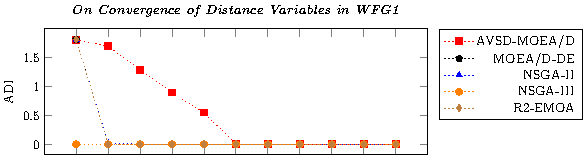
\includegraphics[scale=0.8]{images/Diversity_Long_Term_tikz_WFG1-figure0.eps}\\[0cm]%[-0.14cm] 
 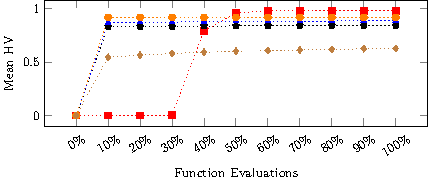
\includegraphics[scale=0.8]{images/Diversity_Long_Term_tikz_WFG1-figure1.eps}\\[0cm]%[-0.14cm] 
\end{tabular}
\caption{Performance of \MOEAS{} for the problems with two objectives considering three ranges for the stopping criterion: 
short-term (first row), middle-term (second row) and long-term (third row).}\label{fig:Performance_time_2obj}
\end{figure}


\subsection{Decision Variable Scalability Analysis}

In order to study the scalability of \VSDMOEA{} in terms of the number of decision variables, all of the algorithms already described were tested with
the same benchmark problems, but considering $50$, $100$, and $250$ variables.
%
Note that in the WFG test problems, the number of position parameters ($k$) and distance parameters ($l$) must be specified.
%
Specifically, the number of distance parameters was set to $42$, $84$, and $210$ when using $50$, $100$ and $250$ variables, respectively.
%
The rest of the decision variables were position parameters, meaning that they were $8$, $16$ and $40$, respectively.
%
Note that increasing the number of variables greatly increases the computing time required.
%
As a result, this study takes into account middle-term executions.
%
%Specifically, the stopping criterion was set to $25,000$ generations.
Specifically, the stopping criterion was set to $2.5 \times 10^6$ function evaluations.
%
Figures~\ref{fig:variable-decision-scalability-2obj} and~\ref{fig:variable-decision-scalability-3obj} 
show the mean \HV{} ratio for the four algorithms tested,
considering the problems with two and three objectives, respectively.
%
As expected, the \HV{} ratio decreases as the number of variables increases.
%
In the two-objective case, the deterioration is similar in every algorithm, so the superiority of \VSDMOEA{} is clear regardless of the number of 
variables.
%
In contrast, in the three-objective case, the deterioration of \VSDMOEA{} is higher than for \RMOEA{} and \MOEAD{}.
%
In fact, when considering $250$ variables, the performance of \VSDMOEA{} is just slightly superior to that of \RMOEA{}.


In order to better understand this behavior, we selected problems WFG1 to WFG7.
%
The WFG test problems divide the variables into two kinds of parameters (this framework uses the term parameter instead of 
variable): the distance parameters and the position parameters.
%
Note that a parameter $i$ is a distance parameter when for all $\vec{\mathbf{x}}$, modifying $x_i$ results in a new solution 
that dominates $\vec{\mathbf{x}}$, is equivalent to $\vec{\mathbf{x}}$, or is dominated by $\vec{\mathbf{x}}$.
%
However, if $i$ is a position parameter, modifying $x_i$ in $\vec{\mathbf{x}}$ always results in a vector that is incomparable or 
equivalent to $\vec{\mathbf{x}}$~\cite{huband2005scalable}.
%
Additionally, note that we selected problems WFG1-WFG7 because their distance parameter values associated to all Pareto optimal solutions 
have exactly the same values:
%
\begin{equation}
   x_{i=k+1:n} = 2i \times 0.35
\end{equation}
%
This is very important because it has been shown that for these cases, state-of-the-art
\MOEAS{} might provoke a quick convergence in \textit{distance parameters}, resulting in an effect that is similar to premature convergence
in the single-objective case~\cite{Joel:GDE3_CEC09}.

%\begin{figure}[t]
%\centering
%\includegraphics[scale=0.85]{Images/Graphic-Diversity_2obj_tikz-figure1.eps}
%\caption{Evolution of ADI for problems WFG1-WFG7 with two objectives considering only the distance variables}\label{fig:Diversity_2obj}
%\end{figure}

For each algorithm, we calculated the average Euclidean distance among individuals (ADI) in the population by considering only 
the distance parameters.
%
Figures~\ref{fig:Diversity_2obj} and~\ref{fig:Diversity_3obj} show how the ADI evolves for the two-objective and three-objective problems.
%
The behavior of \NSGAII{} and \MOEAD{} --- which are not included --- is similar to that of \RMOEA{} in terms of how the ADI evolves. 
%
Thus, to avoid saturating these Figures, only the information for \VSDMOEA{} and \RMOEA{} with 50, 100 and 250 variables is shown.
%
The first obvious fact is that \VSDMOEA{} converges much slower than \RMOEA{}.
%
Accordingly, the difference between the diversity maintained in the first generation and that maintained after 10\% of the execution,
is much larger in \RMOEA{} than in \VSDMOEA{}.
%
In the case of \VSDMOEA{}, the decrease in ADI is quite linear until the halfway point of the execution.
%
This is due to the way in which the threshold distance value ($D_t$) is calculated.
%
Additionally, a closer inspection of the data reveals other important aspects that must be discussed. 
%
In the two-objective case, increasing the number of variables causes the diversity in the \RMOEA{} to increase slightly.
%
However, the amount of diversity is low even when using 250 variables, meaning that incorporating mechanisms to increase diversity --- as is done in \VSDMOEA{} ---
is very helpful.
%
In contrast, in the three-objective case, the amount of diversity in \RMOEA{} is not as low.
%
Moreover, increasing the number of variables yields a significant increase in the resulting ADI, meaning that in this case,
fast convergence is not an important issue.
%
These results show that, as the number of objectives and variables increases, \MOEAS{} tend to maintain a higher variable space diversity
in an implicit way, meaning that explicitly controlling the variable space diversity is probably not as important.
%

Finally, it is worth noting that we selected some problems to conduct long-term executions with 250 variables.
%
\VSDMOEA{} was able to further improve the results when using long-term executions, while the other state-of-the-art algorithms did not yield significant improvements.
%
This probably means that as technology evolves, allowing longer executions to be carried out in reasonable time frames,
the incorporation of explicit control of diversity will be even more important.
%
Note that this also happens in the single-objective case, where the benefits of explicitly controlling diversity appears only when using executions lasting
several weeks when dealing with large instances of the Traveling Salesman Problem~\cite{segura2015novel}.
%

%\begin{figure}[t]
%\centering
%\includegraphics[scale=0.85]{Images/Graphic-Diversity_3obj_tikz-figure1.eps}
%\caption{Evolution of ADI for problems WFG1-WFG7 with three objectives considering only the distance variables}\label{fig:Diversity_3obj}
%\end{figure}



\begin{figure}[t]
\centering
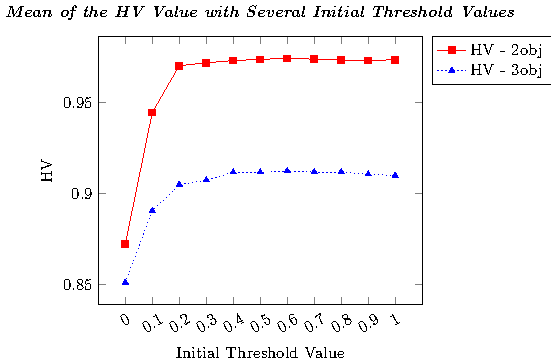
\includegraphics[scale=0.85]{images/Graphic-Initial-Distance_tikz-figure0.eps} \\
\caption{Mean of \HV{} values taking into account all the problems with several initial threshold values}\label{fig:Initial-distance-factor}
\end{figure}



\begin{figure}[t]
\centering
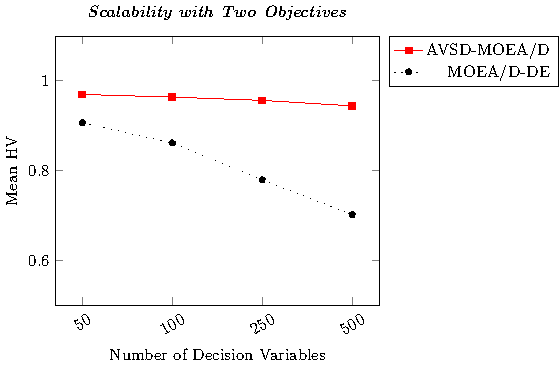
\includegraphics[scale=0.85]{images/Graphic-Scalability-2obj_tikz-figure0.eps}
\caption{Mean of the \HV{} ratio for 35 runs for the two-objective problems considering different numbers of variables}\label{fig:variable-decision-scalability-2obj}
\end{figure}

\begin{figure}[t]
\centering
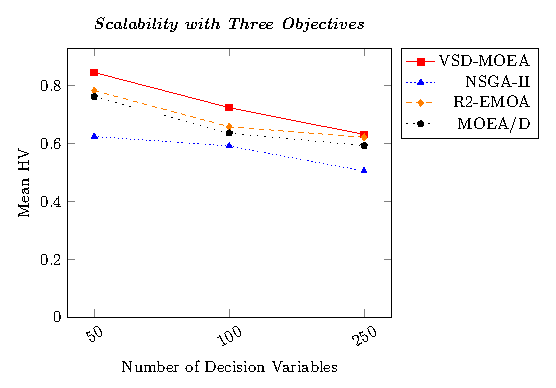
\includegraphics[scale=0.85]{images/Graphic-Scalability-3obj_tikz-figure0.eps}
\caption{Mean of the \HV{} ratio for 35 runs for the three-objective problems considering different numbers of variables} \label{fig:variable-decision-scalability-3obj}
\end{figure}


\subsection{Analysis of the Initial Threshold Value}

One of the disadvantages of including a strategy for controlling diversity is that this is usually done at the expense of
incorporating additional parameters in the \EA{} designed.
%
In the case of \VSDMOEA{}, the initial threshold value ($D_I$) must be set.
%
Note that in all the previous experiments, $D_I = 0.4$ was used.
%
This value was selected based on some preliminary experiments.
%
This section is devoted to analyzing the performance of \VSDMOEA{} when using different $D_I$ values. 
%
Note that, since normalized distances are used, the maximum difference that can appear is $1$.
%
Additionally, note that when $D_I$ is set to 0, no individual is penalized on the basis of its decision
variable space diversity contribution,
so \VSDMOEA{} would behave like a more traditional \MOEA{}.
%
As a result, the values $D_I = \{0.0, 0.1, 0.2, 0.3, 0.4, 0.5, 0.6, 0.7, 0.8, 0.9\}$ were tested.
%
As in previous experiments, the whole set of benchmark problems was used and
the stopping criterion was set to $2.5 \times 10^7$ function evaluations.

Figure~\ref{fig:Initial-distance-factor} shows the mean \HV{} ratio obtained for both the two-objective 
and the three-objective case.
%
Note that even when $D_I$ is set to $0$, \VSDMOEA{} yielded better \HV{} ratios than other 
state-of-the-art algorithms (see Tables~\ref{tab:StatisticsHV_2obj} and~\ref{tab:StatisticsHV_3obj}).
%
Specifically, the values were $0.912$ and $0.893$ for two and three objectives, respectively.
%
This means that the novel density estimator put forth in this paper is indeed helpful.
%
However, the increase in performance when using other $D_I$ values is clear.
%
The \HV{} ratio obtained quickly increases as higher $D_I$ values up to $0.4$ are used.
%
Then, with values in the range $[0.5, 0.9]$, the performance decreases slightly.
%
There is a large range of values where the performance is very good, meaning that 
the behavior of \VSDMOEA{} is quite robust.
%
Thus, properly setting this parameter is not a complex task.

